%%%%%%%%%%%%%%%%%%%%%%%%%%%%%%%%%%%%%%%%%%%%%%%%%%%%%%%%%%%%%%%%%%%%%%%%%%%
%
% Generic template for TFC/TFM/TFG/Tesis
%
% $Id: book.tex,v 1.8 2013/11/27 00:35:13 macias Exp $
%
% By:
%  + Javier Mac�as-Guarasa. 
%    Departamento de Electr�nica
%    Universidad de Alcal�
%  + Roberto Barra-Chicote. 
%    Departamento de Ingenier�a Electr�nica
%    Universidad Polit�cnica de Madrid   
% 
% Based on original sources by Roberto Barra, Manuel Oca�a, Jes�s Nuevo,
% Pedro Revenga, Fernando Herr�nz and Noelia Hern�ndez. Thanks a lot to
% all of them, and to the many anonymous contributors found (thanks to
% google) that provided help in setting all this up.
%
% If you think you can add pieces of relevant/useful examples,
% improvements, please contact us at (macias@depeca.uah.es)
%
% Copyleft 2013
%
%%%%%%%%%%%%%%%%%%%%%%%%%%%%%%%%%%%%%%%%%%%%%%%%%%%%%%%%%%%%%%%%%%%%%%%%%%%

% This is for rubber to clean additional files
% rubber: clean book.acn book.acr book.alg book.cod book.ist book.out book.sbl book.slg book.sym

%%%%%%%%%%%%%%%%%%%%%%%%%%%%%%%%%%%%%%%%%%%%%%%%%%%%%%%%%%%%%%%%%%%%%%%%%%%
% BEGIN Preamble and configuration section
%
\documentclass[svgnames,spanish,openright]{book}
%\documentclass[english,openright]{book}
%\documentclass[11pt,english,twoside,openright]{book}

%\usepackage[a4,cam,center]{crop}
%\crop[font=\upshape\mdseries\small\textsf]

\usepackage[latin1]{inputenc} % Para poder escribir con acentos y �.
\usepackage[T1]{fontenc}      % Para que haga bien la ``hyphenation''. No
                              % usar si no es necesario, porque ralentiza muchisimo la compilaci�n.
\usepackage{ae}               % Para que todas las fuentes sean Type1, y ninguna Type3.

\usepackage[spanish, english]{babel}

% Use this if you want to include pdf files in the final document
\usepackage[final]{pdfpages}

% Use this if you want to delete headers and footers in empty pages
\usepackage{emptypage}

%\usepackage[nottoc]{tocbibind}
\usepackage{tocbibind}

% To draw rectagles in tfm cover
\usepackage{tikz}

\usepackage{listings}
\usepackage{longtable}
\usepackage{afterpage}

\usepackage{xspace}
\usepackage{verbatim}
\usepackage{moreverb}
\usepackage{multicol}
\usepackage{amsmath}
\usepackage{eurosym}
\usepackage{subfigure}
\usepackage{multirow}
\usepackage{fancyhdr}
\usepackage{makeidx}
\usepackage{rotating}
\usepackage{supertabular}
\usepackage{hhline}
\usepackage{array}
\usepackage[noadjust]{cite}      % Written by Donald Arseneau
                        % V1.6 and later of IEEEtran pre-defines the format
                        % of the cite.sty package \cite{} output to follow
                        % that of IEEE. Loading the cite package will
                        % result in citation numbers being automatically
                        % sorted and properly "ranged". i.e.,
                        % [1], [9], [2], [7], [5], [6]
                        % (without using cite.sty)
                        % will become:
                        % [1], [2], [5]--[7], [9] (using cite.sty)
                        % cite.sty's \cite will automatically add leading
                        % space, if needed. Use cite.sty's noadjust option
                        % (cite.sty V3.8 and later) if you want to turn this
                        % off. cite.sty is already installed on most LaTeX
                        % systems. The latest version can be obtained at:
                        % http://www.ctan.org/tex-archive/macros/latex/contrib/supported/cite/


\usepackage{color}

%\usepackage[authoryear]{natbib}
% \makeatletter
% \let\NAT@parse\undefined
% \makeatother
% \usepackage{natbib}

\usepackage{geometry}
\geometry{verbose,a4paper,tmargin=2.5cm,bmargin=2.5cm,lmargin=2.5cm,rmargin=2.5cm}
%\geometry{paperwidth=210mm,paperheight=297mm}

\usepackage[
ps2pdf,                %%% hyper-references for ps2pdf
bookmarks=true,%                   %%% generate bookmarks ...
bookmarksnumbered=true,            %%% ... with numbers
hypertexnames=false,               %%% needed for correct links to
                                %%% figures!!!
%hypertexnames=true,               %%% needed for correct links on pagebackrefs!!!
breaklinks=true,                   %%% breaks lines, but links are very small
%pagebackref=true,
%linktocpage=true,                 %%% enlace en el numero de p�gina.
linktoc=all,
colorlinks=true,
linkcolor=azul,    
citecolor=verde,
urlcolor=azul,                     %%% texto  con color
linkbordercolor={0 0 1},           %%% blue frames around links
pdfborder={0 0 112.0}              %%% border-width of frames 
]{hyperref}                        %%% will be multiplied with 0.009 by ps2pdf


% Para numerar las \subsubsection
\setcounter{secnumdepth}{5}
%para hacer que las \subsubsection aparezcan en el indice
\setcounter{tocdepth}{5}
%\setcounter{lofdepth}{2}
\setcounter{table}{1}
\setcounter{figure}{1}
\setcounter{secnumdepth}{4}


\setlength{\parskip}{1ex plus 0.5ex minus 0.2ex}


\usepackage{multirow}

\usepackage{setspace}
% \renewcommand{\baselinestretch}{10}
\newcommand{\mycaptiontable}[1]{
\begin{spacing}{0.6}
  %\vspace{0.5cm}
  \begin{quote}
    %\begin{center}
            {{Table} \thechapter.\arabic{table}: #1}
    %\end{center}
  \end{quote}
  %\vspace{1cm}
  \end{spacing}
  \stepcounter{table}
}

\newcommand{\mycaptionfigure}[1]{
  %\vspace{0.5cm}
  \begin{spacing}{0.6}
  \begin{quote}
    %\begin{center}
            {{Figure} \thechapter.\arabic{figure}: #1}
    %\end{center}
  \end{quote}
  %\vspace{1cm}
  \end{spacing}
  \stepcounter{figure}
}

% \newlength{\myVSpace}% the height of the box
% \setlength{\myVSpace}{0ex}% the default, 
% \newcommand\xstrut{\raisebox{-.5\myVSpace}% symmetric behaviour, 
%   {\rule{0pt}{\myVSpace}}%
% }

\usepackage{amsmath}

\usepackage{courier}

%***************************************************************************
%***************************************************************************
%***************************************************************************
\usepackage{multirow}
\usepackage{rotating}
\usepackage{setspace, amssymb, amsmath, epsfig, multirow, colortbl, tabularx, subfigure}%
% For acronym package:
% If footnote is specified, text will be included in a footnote
% If printonlyused is specified, only used acronyms will be included
% I use the acronym sty under the sty directory as I needed the newest version
%\usepackage[footnote,printonlyused,withpage]{acronym} 
%\usepackage[printonlyused]{sty/acronym}

% Mejor que el acronym es glossaries
\usepackage[acronym,shortcuts,nomain]{glossaries}

% ifthen to allow using language dependent settings
\usepackage{ifthen}

\newcommand{\clearemptydoublepage}{\newpage{\pagestyle{empty}\cleardoublepage}}


\pagestyle{fancy}

% Pantone 160
%\definecolor{headingPortadaTFM}{RGB}{158,84,10}
% Pantone 160C (this is supposed to be the correct one, but it looks horrible in screen)
%\definecolor{headingPortadaTFM}{RGB}{161,86,28}
% Captured color in screen (this looks ok on screen)
\definecolor{headingPortadaTFM}{RGB}{152,118,52}
\definecolor{textoHeadingPortadaTFM}{RGB}{208,205,102}

\definecolor{azul}{rgb}{0,0,1}
\definecolor{verde}{rgb}{0,0.5,0}
\definecolor{rojo}{rgb}{1,0,0}
\definecolor{cyan}{rgb}{0,0.75,0.75}
\definecolor{magenta}{rgb}{0.75,0,0.75}
\definecolor{amarillo}{rgb}{0.75,0.75,0}
\definecolor{gris}{rgb}{0.25,0.25,0.25}
\definecolor{r}{rgb}{0,0,1}
\definecolor{g}{rgb}{0,1,0}
\definecolor{b}{rgb}{1,0,0}
\definecolor{c}{rgb}{0,1,1}
\definecolor{m}{rgb}{1,0,1}
\definecolor{y}{rgb}{1,1,0}
\definecolor{w}{rgb}{1,1,1}
\definecolor{k}{rgb}{0,0,0}
\definecolor{azulE}{rgb}{0,0.3984,0.5977}
\definecolor{amarilloE}{rgb}{0.9961,0.7969,0}
\definecolor{blanco}{rgb}{1,1,1}
\definecolor{burdeos}{rgb}{1,0,0.95}


\providecommand\phantomsection{}
\onehalfspacing
\sloppy  %better line breaks

\renewcommand{\chaptermark}[1]{\markboth{\chaptername\ \thechapter.\ #1}{}}
\renewcommand{\sectionmark}[1]{\markright{\thesection\ #1}{}}



\fancyhf{}

\fancyhead[LE,RO]{\bfseries\thepage}
\fancyhead[LO]{\bfseries\rightmark}
\fancyhead[RE]{\bfseries\leftmark}

\renewcommand{\headrulewidth}{0.5pt}
\renewcommand{\footrulewidth}{0pt}
\addtolength{\headheight}{3.5pt}
\fancypagestyle{plain}{\fancyhead{}  
  \renewcommand{\headrulewidth}{0pt}}

%\makeglossaries

\fancypagestyle{myplain}
{
  \fancyhf{}
  \renewcommand\headrulewidth{0pt}
  \renewcommand\footrulewidth{0pt}
  \fancyfoot[C]{\thepage}
}

% To set background image in TFMs front and back pages
\usepackage[pages=some]{sty/background}

\backgroundsetup{ scale=1, angle=0, opacity=.1, color=pink,
  contents={\includegraphics[width=.7\paperwidth]{logos/logoEPS-UAH.jpg}}, vshift=-50pt,  hshift=0pt }

\makeatletter
\newcommand*{\cleartoleftpage}{%
  \clearpage
    \if@twoside
    \ifodd\c@page
      \hbox{}\newpage
      \if@twocolumn
        \hbox{}\newpage
      \fi
    \fi
  \fi
}
\makeatother
    % All definitions, packages, etc. DO NOT
                               % TOUCH THIS LINE 
                               
%%%%%%%%%%%%%%%%%%%%%%%%%%%%%%%%%%%%%%%%%%%%%%%%%%%%%%%%%%%%%%%%%%%%%%%%%%%
%
% Generic template for TFC/TFM/TFG/Tesis
%
% $Id: myconfig.tex,v 1.4 2013/11/05 00:42:41 macias Exp $
%
% By:
%  + Javier Mac�as-Guarasa. 
%    Departamento de Electr�nica
%    Universidad de Alcal�
%  + Roberto Barra-Chicote. 
%    Departamento de Ingenier�a Electr�nica
%    Universidad Polit�cnica de Madrid   
% 
% Based on original sources by Roberto Barra, Manuel Oca�a, Jes�s Nuevo,
% Pedro Revenga, Fernando Herr�nz and Noelia Hern�ndez. Thanks a lot to
% all of them, and to the many anonymous contributors found (thanks to
% google) that provided help in setting all this up.
%
% If you think you can add pieces of relevant/useful examples,
% improvements, please contact us at (macias@depeca.uah.es)
%
% Copyleft 2013
%
%%%%%%%%%%%%%%%%%%%%%%%%%%%%%%%%%%%%%%%%%%%%%%%%%%%%%%%%%%%%%%%%%%%%%%%%%%%

%%%%%%%%%%%%%%%%%%%%%%%%%%%%%%%%%%%%%%%%%%%%%%%%%%%%%%%%%%%%%%%%%%%%%%%%%%% 
%
% Contents of this file:
% + Definition of variables controlling compilation flavours
% + Definition of your own commands (samples provided)
%
% You must edit it to suit to your specific case
%
% Specially important are the definition of your variables (title of the
% book, your degree, author name, email, advisors, keywords (in Spanish
% and English), year, ... They will be used in generating the adequate
% front and cover pages, automagically.
%
%%%%%%%%%%%%%%%%%%%%%%%%%%%%%%%%%%%%%%%%%%%%%%%%%%%%%%%%%%%%%%%%%%%%%%%%%%% 

%%%%%%%%%%%%%%%%%%%%%%%%%%%%%%%%%%%%%%%%%%%%%%%%%%%%%%%%%%%%%%%%%%%%%%%%%%% 
% BEGIN Set my own variables (control compilation for different flavours)

% Control language specific modifications
% This can be english or spanish
\newcommand{\mybooklanguage}{spanish}

% Control compilation flavour (for PFCs, TFMs, TFGs, Thesis, etc...)
% Degree (titulaci�n), can be:
% IT    - Ingenier�a de Telecomunicaci�n
% IE    - Ingenier�a Electr�nica
% ITTSE - Ingenier�a T�cnica de Telecomunicaci�n, Sistemas Electr�nicos
% ITTST - Ingenier�a T�cnica de Telecomunicaci�n, Sistemas de Telecomunicaci�n
% ITI   - Ingenier�a T�cnica Industrial, Electr�nica Industrial 
% GIEC  - Grado en Ingenier�a Electr�nica de Comunicaciones
% GIEAI - Grado en Ingenier�a en Electr�nica y Autom�tica Industrial
% GIST  - Grado en Ingenier�a en Sistemas de Telecomunicaci�n
% GITT  - Grado en Ingenier�a en Tecnolog�as de la Telecomunicaci�n
% GIT   - Grado en Ingenier�a Telem�tica
% GIC   - Grado en Ingenier�a de Computadores
% GII   - Grado en Ingenier�a Inform�tica
% GSI   - Grado en Sistemas de Informaci�n
% MUSEA - M�ster Universitario en Sistemas Electr�nicos Avanzados. Sistemas Inteligentes
% PHD   - Doctorado
\newcommand{\mydegree}{GIEC}

% General document information
\newcommand{\mybooktitle}{Title of the pfc/tfm/tfg/tesis}
\newcommand{\mybookauthor}{Full name of author}
\newcommand{\mybookemail}{autor@depeca.uah.es}
\newcommand{\mybookadvisors}{Full name of advisors}
\newcommand{\mybookyear}{Year of the examination}
\newcommand{\mybookkeywords}{First, second, third, fourth and fifth (up to a maximum of five)}
\newcommand{\mybookpalabrasclave}{Primera, segunda, tercera, cuarta y quinta (m�ximo de cinco)}

% END Set my own variables (control compilation for different flavours)
%%%%%%%%%%%%%%%%%%%%%%%%%%%%%%%%%%%%%%%%%%%%%%%%%%%%%%%%%%%%%%%%%%%%%%%%%%% 

%%%%%%%%%%%%%%%%%%%%%%%%%%%%%%%%%%%%%%%%%%%%%%%%%%%%%%%%%%%%%%%%%%%%%%%%%%% 
% BEGIN My own commands section 
% Define your own commands here

% This one is to define a specific format for english text in a Spanish
% document
\DeclareRobustCommand{\texten}[1]{\textit{#1}}

% Various examples
\newcommand{\circulo}{\large $\circ$}
\newcommand{\asterisco}{$\ast$}
\newcommand{\cuadrado}{\tiny $\square$}
\newcommand{\triangulo}{\scriptsize $\vartriangle$}
\newcommand{\triangv}{\scriptsize $\triangledown$}
\newcommand{\diamante}{\large $\diamond$}

\newcommand{\new}[1]{\textcolor{magenta}{#1 }}
\newcommand{\argmax}[1]{\underset{#1}{\operatorname{argmax}}}

% END My own commands section 
%%%%%%%%%%%%%%%%%%%%%%%%%%%%%%%%%%%%%%%%%%%%%%%%%%%%%%%%%%%%%%%%%%%%%%%%%%% 

%%% Local Variables:
%%% TeX-master: "../book"
%%% End:


    % EDIT IT! to set your specific settings!

% Define a new glossary type for symbols used in equations
\newglossary[slg]{symbols}{sym}{sbl}{List of Symbols}


\makeglossaries
  % EDIT IT to include your glossaries!

%%%%%%%%%%%%%%%%%%%%%%%%%%%%%%%%%%%%%%%%%%%%%%%%%%%%%%%%%%%%%%%%%%%%%%%%%%%
%
% Generic template for TFC/TFM/TFG/Tesis
%
% $Id: postamble.tex,v 1.21 2020/03/24 17:18:25 macias Exp $
%
% By:
%  + Javier Macías-Guarasa. 
%    Departamento de Electrónica
%    Universidad de Alcalá
%  + Roberto Barra-Chicote. 
%    Departamento de Ingeniería Electrónica
%    Universidad Politécnica de Madrid   
% 
% Based on original sources by Roberto Barra, Manuel Ocaña, Jesús Nuevo,
% Pedro Revenga, Fernando Herránz and Noelia Hernández. Thanks a lot to
% all of them, and to the many anonymous contributors found (thanks to
% google) that provided help in setting all this up.
%
% See also the additionalContributors.txt file to check the name of
% additional contributors to this work.
%
% If you think you can add pieces of relevant/useful examples,
% improvements, please contact us at (macias@depeca.uah.es)
%
% You can freely use this template and please contribute with
% comments or suggestions!!!
%
%%%%%%%%%%%%%%%%%%%%%%%%%%%%%%%%%%%%%%%%%%%%%%%%%%%%%%%%%%%%%%%%%%%%%%%%%%%

%%%%%%%%%%%%%%%%%%%%%%%%%%%%%%%%%%%%%%%%%%%%%%%%%%%%%%%%%%%%%%%%%%%%%%%%%%%
%
% You should not need to edit this file. Yes, I know the name is not a
% valid word... :-)
%
% Here we define \mydegreefull, \mybookworktype and \mybookworktypefull 
% that will be used by other modules. The decision is based on the
% \mydegree variable set by the user.
%
% In case the \mydegree variable is now known, the module will generate 
% an error message in \mydegreefull and \mybookworktypefull, but will 
% generate a valid \mybookworktype, to be able to generate front and
% cover pages (TFG by default)
%
%%%%%%%%%%%%%%%%%%%%%%%%%%%%%%%%%%%%%%%%%%%%%%%%%%%%%%%%%%%%%%%%%%%%%%%%%%%

\ifthenelse{\equal{\mybooklanguage}{spanish}}
{
\usepackage[spanish]{babel}
\newcommand{\mybookFullAffiliation}{Grupo de investigación \mybookresearchgroup \\ \mybookdepartment \\ \mybookuniversity} 
\newcommand{\mybooktitle}{\mybooktitlespanish}
} 
{
\usepackage[english]{babel}
\newcommand{\mybookFullAffiliation}{\mybookresearchgroup Research Group \\ \mybookdepartmentEnglish \\ \mybookuniversity} 
\newcommand{\mybooktitle}{\mybooktitleenglish}
}

\ifthenelse{\equal{\mybooklanguage}{spanish}}
{
\newcommand{\andOrY}{y} 
} 
{
\newcommand{\andOrY}{and} 
}

% Gender issues
\ifthenelse{\equal{\mybookAcademicTutorGender}{male}}     
{                                                       
\newcommand{\donOrDonaTutor}{D.}
\newcommand{\drOrDraTutor}{Dr.}
}
{
\newcommand{\donOrDonaTutor}{Dª.}
\newcommand{\drOrDraTutor}{Dra.}
}

\ifthenelse{\equal{\mybookCoTutorGender}{male}}     
{                                                       
\newcommand{\donOrDonaCoTutor}{D.}
\newcommand{\drOrDraCoTutor}{Dr.}
}
{
\newcommand{\donOrDonaCoTutor}{Dª.}
\newcommand{\drOrDraCoTutor}{Dra.}
}

\ifthenelse{\equal{\mybookauthorgender}{male}}     
{                                                       
\newcommand{\donOrDonaAutor}{D.}
}
{
\newcommand{\donOrDonaAutor}{Dª.}
}

% Set name of advisors and define words depending on singular/plural
\ifthenelse{\equal{\mybookNameCoTutor}{}}
{
\newcommand{\mybookadvisors}{\mybookNameAcademicTutor{}}
\newcommand{\mybookadvisorsConDon}{\donOrDonaTutor{} \mybookNameAcademicTutor{}}
\newcommand{\mybookadvisorsConDr}{\drOrDraTutor{} \mybookNameAcademicTutor{}}
\ifthenelse{\equal{\mybookAcademicTutorGender}{male}}     
{                                                       
\newcommand{\directorOrdirectora}{director}
\newcommand{\mybookTutorOrTutores}{tutor}
\newcommand{\mybookTutor}{tutor}
}
{
\newcommand{\directorOrdirectora}{directora}
\newcommand{\mybookTutorOrTutores}{tutora}
\newcommand{\mybookTutor}{tutora}
}
\newcommand{\mybookDirectorOrDirectores}{\directorOrdirectora}
\newcommand{\mybookAdvisorOrAdvisors}{advisor}
\newcommand{\mybookAdvisor}{advisor}
\newcommand{\mybookCoAdvisor}{co-advisor}
\newcommand{\mybookDaOrDan}{da}
\newcommand{\mybookEmiteOrEmiten}{emite}
\newcommand{\mybookElOrLos}{El}
\newcommand{\mybookSuOrSus}{su}
\newcommand{\mybookDelOrDeLos}{del}
\newcommand{\mybookHagoOrHacemos}{hago}
}
{
\newcommand{\mybookadvisors}{\mybookNameAcademicTutor{} \andOrY{} \mybookNameCoTutor{}}
\newcommand{\mybookadvisorsConDon}{\donOrDonaTutor{} \mybookNameAcademicTutor{} \andOrY{} \donOrDonaCoTutor{} \mybookNameCoTutor{}}
\newcommand{\mybookadvisorsConDr}{\drOrDraTutor{} \mybookNameAcademicTutor{}\\\drOrDraCoTutor{} \mybookNameCoTutor{}}

\newcommand{\mybookDirectorOrDirectores}{directores}
\newcommand{\mybookAdvisorOrAdvisors}{advisors}
\newcommand{\mybookAdvisor}{advisor}
\newcommand{\mybookCoAdvisor}{co-advisor}
\newcommand{\mybookDaOrDan}{dan}
\newcommand{\mybookEmiteOrEmiten}{emiten}
\newcommand{\mybookTutorOrTutores}{tutores}


\ifthenelse{\equal{\mybookAcademicTutorGender}{male}}     
{                                                       
\newcommand{\directorOrdirectora}{director}
\newcommand{\mybookTutor}{tutor}
}
{
\newcommand{\directorOrdirectora}{directora}
\newcommand{\mybookTutor}{tutora}
}

\ifthenelse{\equal{\mybookCoTutorGender}{male}}     
{                                                       
\newcommand{\mybookCoTutor}{cotutor}
}
{
\newcommand{\mybookCoTutor}{cotutora}
}


\newcommand{\mybookElOrLos}{Los}
\newcommand{\mybookSuOrSus}{Su}
\newcommand{\mybookDelOrDeLos}{de los}
\newcommand{\mybookHagoOrHacemos}{hacemos}
}

% Set Autor/Autora field
\ifthenelse{\equal{\mybookauthorgender}{male}}     
{                                                       
\newcommand{\mybookAutorOrAutora}{autor}                
\newcommand{\mybookElOrLa}{el}                
\newcommand{\mybookAlOrALa}{al}                
\newcommand{\mybookDelOrDeLa}{del}                
\newcommand{\mybookDonOrDona}{D}                
\newcommand{\mybookNotificadoOrNotificada}{notificado}                
\newcommand{\mybookAdscritoOrAdscrita}{adscrito}                
\newcommand{\mybookAlumnoOrAlumna}{alumno}                
}                                               
{
\newcommand{\mybookAutorOrAutora}{autora}                
\newcommand{\mybookElOrLa}{la}                
\newcommand{\mybookAlOrALa}{a la}                
\newcommand{\mybookDelOrDeLa}{de la}                
\newcommand{\mybookDonOrDona}{Dª}                
\newcommand{\mybookNotificadoOrNotificada}{notificada}    
\newcommand{\mybookAdscritoOrAdscrita}{adscrita}                
\newcommand{\mybookAlumnoOrAlumna}{alumna}                            
}

% Set degree name and type of document, depending on the user defined degree
\ifthenelse{\equal{\mydegree}{IT}}
{
  \newcommand{\mydegreefull}{Ingeniería de Telecomunicación}
  \newcommand{\mybookworktype}{TFC}
  \ifthenelse{\equal{\mybooklanguage}{spanish}}
  {
    \newcommand{\mybookworktypefull}{Trabajo Fin de Carrera}
  }
  {
    % This could be translated. I'm leaving this in Spanish...
    % \newcommand{\mybookworktypefull}{Master's Thesis}
    \newcommand{\mybookworktypefull}{Trabajo Fin de Carrera}
  }
}
{
  \ifthenelse{\equal{\mydegree}{IE}}
  {
    \newcommand{\mydegreefull}{Ingeniería Electrónica}
    \newcommand{\mybookworktype}{TFC}
    \ifthenelse{\equal{\mybooklanguage}{spanish}}
    {
      \newcommand{\mybookworktypefull}{Trabajo Fin de Carrera}
    }
    {
      % This could be translated. I'm leaving this in Spanish...
      % \newcommand{\mybookworktypefull}{Master's Thesis}
      \newcommand{\mybookworktypefull}{Trabajo Fin de Carrera}
    }
  }
  {
    \ifthenelse{\equal{\mydegree}{ITTSE}}
    {
      \newcommand{\mydegreefull}{Ingeniería Técnica de Telecomunicación, especialidad en Sistemas Electrónicos}
      \newcommand{\mybookworktype}{TFC}
      \ifthenelse{\equal{\mybooklanguage}{spanish}}
      {
        \newcommand{\mybookworktypefull}{Trabajo Fin de Carrera}
      }
      {
        % This could be translated. I'm leaving this in Spanish...
        % \newcommand{\mybookworktypefull}{Bachelor's Thesis}
        \newcommand{\mybookworktypefull}{Trabajo Fin de Carrera}
      }
    }
    {
      \ifthenelse{\equal{\mydegree}{ITTST}}
      {
        \newcommand{\mydegreefull}{Ingeniería Técnica de Telecomunicación, especialidad en Sistemas de Telecomunicación}
      \newcommand{\mybookworktype}{TFC}
        \ifthenelse{\equal{\mybooklanguage}{spanish}}
        {
          \newcommand{\mybookworktypefull}{Trabajo Fin de Carrera}
        }
        {
          % This could be translated. I'm leaving this in Spanish...
          % \newcommand{\mybookworktypefull}{Bachelor's Thesis}
          \newcommand{\mybookworktypefull}{Trabajo Fin de Carrera}
        }
      }
      {
        \ifthenelse{\equal{\mydegree}{ITI}}
        {
          \newcommand{\mydegreefull}{Ingeniería Técnica Industrial, especialidad en Electrónica Industrial}
          \newcommand{\mybookworktype}{TFC}
          \ifthenelse{\equal{\mybooklanguage}{spanish}}
          {
            \newcommand{\mybookworktypefull}{Trabajo Fin de Carrera}
          }
          {
            % This could be translated. I'm leaving this in Spanish...
            % \newcommand{\mybookworktypefull}{Bachelor's Thesis}
            \newcommand{\mybookworktypefull}{Trabajo Fin de Carrera}
          }
        }
        {
          \ifthenelse{\equal{\mydegree}{GIEC}}
          {
            \newcommand{\mydegreefull}{Grado en Ingeniería Electrónica de Comunicaciones}
            \newcommand{\mybookworktype}{TFG}
            \ifthenelse{\equal{\mybooklanguage}{spanish}}
            {
              \newcommand{\mybookworktypefull}{Trabajo Fin de Grado}
            }
            {
              % This could be translated. I'm leaving this in Spanish...
              % \newcommand{\mybookworktypefull}{Bachelor's Thesis}
              \newcommand{\mybookworktypefull}{Trabajo Fin de Grado}
            }
          }
          {
            \ifthenelse{\equal{\mydegree}{GIEAI}}
            {
              \newcommand{\mydegreefull}{Grado en Ingeniería en Electrónica y Automática Industrial}
              \newcommand{\mybookworktype}{TFG}
              \ifthenelse{\equal{\mybooklanguage}{spanish}}
              {
                \newcommand{\mybookworktypefull}{Trabajo Fin de Grado}
              }
              {
                % This could be translated. I'm leaving this in Spanish...
                % \newcommand{\mybookworktypefull}{Bachelor's Thesis}
                \newcommand{\mybookworktypefull}{Trabajo Fin de Grado}
              }
            }
            {
              \ifthenelse{\equal{\mydegree}{GIST}}
              {
                \newcommand{\mydegreefull}{Grado en Ingeniería en Sistemas de Telecomunicación}
                \newcommand{\mybookworktype}{TFG}
                \ifthenelse{\equal{\mybooklanguage}{spanish}}
                {
                  \newcommand{\mybookworktypefull}{Trabajo Fin de Grado}
                }
                {
                  % This could be translated. I'm leaving this in Spanish...
                  % \newcommand{\mybookworktypefull}{Bachelor's Thesis}
                  \newcommand{\mybookworktypefull}{Trabajo Fin de Grado}
                }
              }
              {
                \ifthenelse{\equal{\mydegree}{GITT}}
                {
                  \newcommand{\mydegreefull}{Grado en Ingeniería en Tecnologías de la Telecomunicación}
                  \newcommand{\mybookworktype}{TFG}
                  \ifthenelse{\equal{\mybooklanguage}{spanish}}
                  {
                    \newcommand{\mybookworktypefull}{Trabajo Fin de Grado}
                  }
                  {
                    % This could be translated. I'm leaving this in Spanish...
                    % \newcommand{\mybookworktypefull}{Bachelor's Thesis}
                    \newcommand{\mybookworktypefull}{Trabajo Fin de Grado}
                  }
                }
                {
                  \ifthenelse{\equal{\mydegree}{GIT}}
                  {
                    \newcommand{\mydegreefull}{Grado en Ingeniería Telemática}
                    \newcommand{\mybookworktype}{TFG}
                    \ifthenelse{\equal{\mybooklanguage}{spanish}}
                    {
                      \newcommand{\mybookworktypefull}{Trabajo Fin de Grado}
                    }
                    {
                      % This could be translated. I'm leaving this in Spanish...
                      % \newcommand{\mybookworktypefull}{Bachelor's Thesis}
                      \newcommand{\mybookworktypefull}{Trabajo Fin de Grado}
                    }
                  }
                  {
                    \ifthenelse{\equal{\mydegree}{GIC}}
                    {
                      \newcommand{\mydegreefull}{Grado en Ingeniería de Computadores}
                      \newcommand{\mybookworktype}{TFG}
                      \ifthenelse{\equal{\mybooklanguage}{spanish}}
                      {
                        \newcommand{\mybookworktypefull}{Trabajo Fin de Grado}
                      }
                      {
                        % This could be translated. I'm leaving this in Spanish...
                        % \newcommand{\mybookworktypefull}{Bachelor's Thesis}
                        \newcommand{\mybookworktypefull}{Trabajo Fin de Grado}
                      }
                    }
                    {
                      \ifthenelse{\equal{\mydegree}{GII}}
                      {
                        \newcommand{\mydegreefull}{Grado en Ingeniería Informática}
                        \newcommand{\mybookworktype}{TFG}
                        \ifthenelse{\equal{\mybooklanguage}{spanish}}
                        {
                          \newcommand{\mybookworktypefull}{Trabajo Fin de Grado}
                        }
                        {
                          % This could be translated. I'm leaving this in Spanish...
                          % \newcommand{\mybookworktypefull}{Bachelor's Thesis}
                          \newcommand{\mybookworktypefull}{Trabajo Fin de Grado}
                        }
                      }
                      {
                        \ifthenelse{\equal{\mydegree}{GSI}}
                        {
                          \newcommand{\mydegreefull}{Grado en Sistemas de Información}
                          \newcommand{\mybookworktype}{TFG}
                          \ifthenelse{\equal{\mybooklanguage}{spanish}}
                          {
                            \newcommand{\mybookworktypefull}{Trabajo Fin de Grado}
                          }
                          {
                            % This could be translated. I'm leaving this in Spanish...
                            % \newcommand{\mybookworktypefull}{Bachelor's Thesis}
                            \newcommand{\mybookworktypefull}{Trabajo Fin de Grado}
                          }
                        }
                        {
                          \ifthenelse{\equal{\mydegree}{MUSEA}}
                          {
                            \newcommand{\mydegreefull}{Máster Universitario en Sistemas Electrónicos Avanzados. Sistemas Inteligentes}
                            \newcommand{\mydegreefullwrapped}{Máster Universitario en Sistemas Electrónicos Avanzados\\Sistemas Inteligentes}
                            \newcommand{\mydegreefullwrappedUpcase}{\MakeUppercase{Máster Universitario en}\\\MakeUppercase{Ingeniería de Telecomunicación}}
                            \newcommand{\mybookworktype}{TFM}
                            \ifthenelse{\equal{\mybooklanguage}{spanish}}
                            {
                              \newcommand{\mybookworktypefull}{Trabajo Fin de Máster}
                            }
                            {
                              % This could be translated. I'm leaving this in Spanish...
                              % \newcommand{\mybookworktypefull}{Master's Thesis}
                              \newcommand{\mybookworktypefull}{Trabajo Fin de Máster}
                            }
                          }
                          {
                            \ifthenelse{\equal{\mydegree}{PHDUAH}}
                            {
                              \newcommand{\mydegreefull}{Estudios de Doctorado}
                              \newcommand{\mybookworktype}{PHDUAH}
                              \ifthenelse{\equal{\mybooklanguage}{spanish}}
                              {
                                \newcommand{\mybookworktypefull}{Tesis Doctoral}
                              }
                              {
                                \newcommand{\mybookworktypefull}{Doctoral Thesis}
                              }
                            }
                            {
                              \ifthenelse{\equal{\mydegree}{PHDUPM}}
                              {
                                \newcommand{\mydegreefull}{Doctor Ingeniero de Telecomunicación}
                                \newcommand{\mybookworktype}{PHDUPM}
                                \ifthenelse{\equal{\mybooklanguage}{spanish}}
                                {
                                  \newcommand{\mybookworktypefull}{Tesis Doctoral}
                                }
                                {
                                  \newcommand{\mybookworktypefull}{Doctoral Thesis}
                                }
                              }
                              {
                                \ifthenelse{\equal{\mydegree}{GEINTRARR}}
                                {
                                  \newcommand{\mydegreefull}{GEINTRA Research Report}
                                  \newcommand{\mybookworktype}{GEINTRARR}
                                  \ifthenelse{\equal{\mybooklanguage}{spanish}}
                                  {
                                    \newcommand{\mybookworktypefull}{Informe técnico del Grupo de investigación \mybookresearchgroup{}}
                                  }
                                  {
                                    \newcommand{\mybookworktypefull}{\mybookresearchgroup{} Research Report}
                                  }
                                }
                                {
                                  \ifthenelse{\equal{\mydegree}{MUIT}}
                                  {
                                    \newcommand{\mydegreefull}{Máster Universitario en Ingeniería de Telecomunicación}
                                    \newcommand{\mydegreefullwrapped}{Máster Universitario en Ingeniería de Telecomunicación}
                                    \newcommand{\mydegreefullwrappedUpcase}{\MakeUppercase{Máster Universitario en}\\\MakeUppercase{Ingeniería de Telecomunicación}}
                                    \newcommand{\mybookworktype}{TFM}
                                    \ifthenelse{\equal{\mybooklanguage}{spanish}}
                                    {
                                    \newcommand{\mybookworktypefull}{Trabajo Fin de Máster}
                                    }
                                    {
                                    % This could be translated. I'm leaving this in Spanish...
                                    % \newcommand{\mybookworktypefull}{Master's Thesis}
                                    \newcommand{\mybookworktypefull}{Trabajo Fin de Máster}
                                    }
                                 }
                                 {
                                   \ifthenelse{\equal{\mydegree}{MUII}}
                                   {
                                     \newcommand{\mydegreefull}{Máster Universitario en Ingeniería Industrial}
                                     \newcommand{\mydegreefullwrapped}{Máster Universitario en Ingeniería Industrial}
                                     \newcommand{\mydegreefullwrappedUpcase}{\MakeUppercase{Máster Universitario en}\\\MakeUppercase{Ingeniería Industrial}}
                                     \newcommand{\mybookworktype}{TFM}
                                     \ifthenelse{\equal{\mybooklanguage}{spanish}}
                                     {
                                       \newcommand{\mybookworktypefull}{Trabajo Fin de Máster}
                                     }
                                     {        
                                     % This could be translated. I'm leaving this in Spanish...
                                     % \newcommand{\mybookworktypefull}{Master's Thesis}
                                     \newcommand{\mybookworktypefull}{Trabajo Fin de Máster}
                                     }
                                   }
                                   {
                                     \ifthenelse{\equal{\mydegree}{GITI}}
                                     {
                                       \newcommand{\mydegreefull}{Grado en Ingeniería en Tecnologías Industriales}
                                       \newcommand{\mybookworktype}{TFG}
                                       \ifthenelse{\equal{\mybooklanguage}{spanish}}
                                       {
                                       \newcommand{\mybookworktypefull}{Trabajo Fin de Grado}
                                       }
                                       {
                                       % This could be translated. I'm leaving this in Spanish...
                                       % \newcommand{\mybookworktypefull}{Bachelor's Thesis}
                                       \newcommand{\mybookworktypefull}{Trabajo Fin de Grado}
                                       }
                                     }
                                     {

                                       \ifthenelse{\equal{\mydegree}{GISI}}
                                       {
                                         \newcommand{\mydegreefull}{Grado en Ingeniería en Sistemas de Información}
                                         \newcommand{\mybookworktype}{TFG}
                                         \ifthenelse{\equal{\mybooklanguage}{spanish}}
                                         {
                                           \newcommand{\mybookworktypefull}{Trabajo Fin de Grado}
                                         }
                                         {
                                           % This could be translated. I'm leaving this in Spanish...
                                           % \newcommand{\mybookworktypefull}{Bachelor's Thesis}
                                           \newcommand{\mybookworktypefull}{Trabajo Fin de Grado}
                                         }
                                       }
                                       {
                                         \newcommand{\mybookworktype}{TFG}
                                         \newcommand{\mydegreefull}{ERROR: Defined degree (\mydegree) unknown, check \texttt{config/myconfig.tex}} 
                                         \newcommand{\mybookworktypefull}{ERROR: Defined degree (\mydegree) unknown, check \texttt{config/myconfig.tex}}
                                       }


                                     }
                                   }
                                 }
                               
                                }                               
                              }                          
                            }                          
                          }                          
                        }
                      }
                    }
                  }
                }
              }
            }
          }
        }
      }
    }
  }
}




%%%%%%%%%%%%%%%%%%%%%%%%%%%%%%%%%%%%%%%%%%%%%%%%%%%%%%%%%%%%%%%%%%%%%%%%%%%
% BEGIN Definition of the pdf document information data

\newcommand{\contactauthor}{\mybookauthor~\textless\href{mailto:\mybookemail}{\mybookemail}\textgreater}

% Set keywords for pdf information
\ifthenelse{\equal{\mybooklanguage}{english}}
{
  \newcommand{\keywordsforpdf}{\mybookkeywords}
}
{
  \newcommand{\keywordsforpdf}{\mybookpalabrasclave}
}

\newcommand{\underscoreSpacingFour}{\_\_\_\_}
\newcommand{\spacingFour}{~~~~}

\hypersetup
{
  pdfauthor={\mybookauthor~\textless\href{mailto:\mybookemail}{\mybookemail}\textgreater},
  pdftitle={\mybooktitle},
  pdfsubject={\mydegreefull, \mybookworktypefull},
% Uncomment the English or Spanish version if you wish to hard-code them
%  pdfkeywords={\mybookkeywords, \mybookworktypefull, \mydegreefull},
%  pdfkeywords={\mybookpalabrasclave, \mybookworktypefull, \mydegreefull},
  pdfkeywords={\keywordsforpdf},
  pdfcreator={\LaTeX with hyperref package},
  pdfproducer={rubber},
  pdffitwindow={true},
% This can be set in myconfig.tex
  urlcolor=\myurlcolor,
  linkcolor=\mylinkcolor,
  citecolor=\mycitecolor
}

% END Definition of the pdf document information data
%%%%%%%%%%%%%%%%%%%%%%%%%%%%%%%%%%%%%%%%%%%%%%%%%%%%%%%%%%%%%%%%%%%%%%%%%%%

%%% Local Variables:
%%% TeX-master: "../book"
%%% End:


   % DO NOT TOUCH THIS LINE. Yes, I know,
                               % "postamble" is not a valid word... :-)

% ruta de las im�genes
\graphicspath{{./logos/}{./results/}{./diagrams/}} % Edit this to your
                                % needs. Only logos is really required
%
% END Preamble and configuration section
%%%%%%%%%%%%%%%%%%%%%%%%%%%%%%%%%%%%%%%%%%%%%%%%%%%%%%%%%%%%%%%%%%%%%%%%%%%

%%%%%%%%%%%%%%%%%%%%%%%%%%%%%%%%%%%%%%%%%%%%%%%%%%%%%%%%%%%%%%%%%%%%%%%%%%%
% Let's start with the real stuff
%%%%%%%%%%%%%%%%%%%%%%%%%%%%%%%%%%%%%%%%%%%%%%%%%%%%%%%%%%%%%%%%%%%%%%%%%%%
\begin{document}

%%%%%%%%%%%%%%%%%%%%%%%%%%%%%%%%%%%%%%%%%%%%%%%%%%%%%%%%%%%%%%%%%%%%%%%%%%%
% Now start text and numbering for frontmatter (toc, list of
% tables/figures,...) 
%%%%%%%%%%%%%%%%%%%%%%%%%%%%%%%%%%%%%%%%%%%%%%%%%%%%%%%%%%%%%%%%%%%%%%%%%%%
\frontmatter

%%%%%%%%%%%%%%%%%%%%%%%%%%%%%%%%%%%%%%%%%%%%%%%%%%%%%%%%%%%%%%%%%%%%%%%%%%%
% BEGIN within-document configuration, frontpage and cover pages generation
%

% Set Language dependent issues that must be set after \begin{document}
%%%%%%%%%%%%%%%%%%%%%%%%%%%%%%%%%%%%%%%%%%%%%%%%%%%%%%%%%%%%%%%%%%%%%%%%%%%
%
% Generic template for TFC/TFM/TFG/Tesis
%
% $Id: setlanguagedependentissues.tex,v 1.4 2013/11/04 23:46:21 macias Exp $
%
% By:
%  + Javier Mac�as-Guarasa. 
%    Departamento de Electr�nica
%    Universidad de Alcal�
%  + Roberto Barra-Chicote. 
%    Departamento de Ingenier�a Electr�nica
%    Universidad Polit�cnica de Madrid   
% 
% Based on original sources by Roberto Barra, Manuel Oca�a, Jes�s Nuevo,
% Pedro Revenga, Fernando Herr�nz and Noelia Hern�ndez. Thanks a lot to
% all of them, and to the many anonymous contributors found (thanks to
% google) that provided help in setting all this up.
%
% If you think you can add pieces of relevant/useful examples,
% improvements, please contact us at (macias@depeca.uah.es)
%
% Copyleft 2013
%
%%%%%%%%%%%%%%%%%%%%%%%%%%%%%%%%%%%%%%%%%%%%%%%%%%%%%%%%%%%%%%%%%%%%%%%%%%%

%%%%%%%%%%%%%%%%%%%%%%%%%%%%%%%%%%%%%%%%%%%%%%%%%%%%%%%%%%%%%%%%%%%%%%%%%%%
%
% You should not need to modify this file, unless you want to add
% language specific definitions.
%
%%%%%%%%%%%%%%%%%%%%%%%%%%%%%%%%%%%%%%%%%%%%%%%%%%%%%%%%%%%%%%%%%%%%%%%%%%%

\ifthenelse{\equal{\mybooklanguage}{english}}
{
  \selectlanguage{english}
}
{
  \selectlanguage{spanish}
  
  \renewcommand{\tablename}{Tabla}
  \renewcommand{\listtablename}{�ndice de tablas}
}

%%% Local Variables:
%%% TeX-master: "../book"
%%% End:


 % DO NOT TOUCH THIS LINE/FILE

% This will include front page (if needed), and cover pages. Selection
% of the adequate one is done automagically depending on values set by
% the user in config/myconfig.tex
%%%%%%%%%%%%%%%%%%%%%%%%%%%%%%%%%%%%%%%%%%%%%%%%%%%%%%%%%%%%%%%%%%%%%%%%%%% 
% Defines the cover to be used depending on the type of work (that is
% turn depends on the \mydegree variable
%%%%%%%%%%%%%%%%%%%%%%%%%%%%%%%%%%%%%%%%%%%%%%%%%%%%%%%%%%%%%%%%%%%%%%%%%%%

\ifthenelse{\equal{\mybookworktype}{TFG}}
{
  %%%%%%%%%%%%%%%%%%%%%%%%%%%%%%%%%%%%%%%%%%%%%%%%%%%%%%%%%%%%%%%%%%%%%%%%%%%
%
% Generic template for TFC/TFM/TFG/Tesis
%
% $Id: portada-tfg-uah.tex,v 1.12 2015/06/05 00:10:34 macias Exp $
%
% By:
%  + Javier Mac�as-Guarasa. 
%    Departamento de Electr�nica
%    Universidad de Alcal�
%  + Roberto Barra-Chicote. 
%    Departamento de Ingenier�a Electr�nica
%    Universidad Polit�cnica de Madrid   
% 
% Based on original sources by Roberto Barra, Manuel Oca�a, Jes�s Nuevo,
% Pedro Revenga, Fernando Herr�nz and Noelia Hern�ndez. Thanks a lot to
% all of them, and to the many anonymous contributors found (thanks to
% google) that provided help in setting all this up.
%
% See also the additionalContributors.txt file to check the name of
% additional contributors to this work.
%
% If you think you can add pieces of relevant/useful examples,
% improvements, please contact us at (macias@depeca.uah.es)
%
% You can freely use this template and please contribute with
% comments or suggestions!!!
%
%%%%%%%%%%%%%%%%%%%%%%%%%%%%%%%%%%%%%%%%%%%%%%%%%%%%%%%%%%%%%%%%%%%%%%%%%%%

\thispagestyle{empty}

% To add background watermark
\BgThispage

% Nice example of tikz
% \begin{tikzpicture}[remember picture,overlay]
%   \node [xshift=1cm,yshift=1cm] at (current page.south west)
%   [text width=7cm,fill=red!20,rounded corners,above right]
%   {
%     This is an absolutely positioned text in the
%     lower left corner. No shipout-hackery is used.
%   };
% \end{tikzpicture}

\begin{tikzpicture}[remember picture,overlay]
    \node[yshift=-5cm] at (current page.north west)
      {
        \begin{tikzpicture}[remember picture, overlay]
          \draw[fill=headingPortadaTFG,headingPortadaTFG] (0,0) rectangle (\paperwidth,5cm);
          \node [yshift=3cm, xshift=0.5\paperwidth, font=\Huge, text centered, midway] {\color{textoHeadingPortadaTFM}\textbf{\mybookuniversity}};
          \node [yshift=2cm, xshift=0.5\paperwidth, font=\Huge, text centered, midway] {\color{textoHeadingPortadaTFM}\textbf{\mybookschool}};

        \end{tikzpicture}
      };
   \end{tikzpicture}


\large
\vspace{5cm}
\begin{center}

  % titulaci�n a la que se opta
  \LARGE\textbf{\mydegreefull}

  \vspace{25mm}

  \LARGE\textbf{\mybookworktypefull}

  \LARGE{\mybooktitle}

\vspace{5cm}

\ifthenelse{\equal{\mybooklanguage}{english}}
{
  \textbf{Author:}  \mybookauthor 
}
{
  \textbf{Autor:}  \mybookauthor 
}

\vspace{0.5cm}

% If also director: add corresponding line (mybookDirectors IS NOT DEFINED AS FOR ME (JMG)
%   \ifthenelse{\equal{\mybooklanguage}{english}}
%   {
%     \textbf{\expandafter\makefirstuc\expandafter{\mybookAdvisorOrAdvisors}:} \mybookadvisors
%   }
%   {
%   \textbf{\expandafter\makefirstuc\expandafter{\mybookTutorOrTutores}:}  \mybookadvisors
% %  \textbf{\expandafter\makefirstuc\expandafter{\mybookDirectorOrDirectores}:}  \mybookdirectors
%   }

% ---
  \ifthenelse{\equal{\mybooktutoresseparados}{true}}
{
  \ifthenelse{\equal{\mybooklanguage}{english}}
  {
%    \expandafter\makefirstuc\expandafter{\mybookAdvisorOrAdvisors}: \mybookadvisors
    \textbf{\expandafter\makefirstuc\expandafter{\mybookAdvisor}:} \mybookNameAcademicTutor{}

    \ifthenelse{\equal{\mybookNameCoTutor}{}}
    {
    }
    {
    \textbf{\expandafter\makefirstuc\expandafter{\mybookCoAdvisor}:} \mybookNameCoTutor{}
    }

  }
  {%
%    \expandafter\makefirstuc\expandafter{\mybookDirectorOrDirectores}: \mybookadvisors
%    \expandafter\makefirstuc\expandafter{\mybookTutorOrTutores}: \mybookadvisors
    \textbf{\expandafter\makefirstuc\expandafter{\mybookTutor}:}    \mybookNameAcademicTutor{}

    \ifthenelse{\equal{\mybookNameCoTutor}{}}
    {
    }
    {
    \textbf{\expandafter\makefirstuc\expandafter{\mybookCoTutor}:} \mybookNameCoTutor{}
    }
  }
}
{
  \ifthenelse{\equal{\mybooklanguage}{english}}
  {
    \textbf{\expandafter\makefirstuc\expandafter{\mybookAdvisorOrAdvisors}:} \mybookadvisors
  }
  {
    \textbf{\expandafter\makefirstuc\expandafter{\mybookTutorOrTutores}:} \mybookadvisors
  }
}  


%---


\end{center}

\begin{bottomparagraph}
  \begin{center}
    \huge{\mybookyear}
  \end{center}
\end{bottomparagraph}

%\newpage
\clearemptydoublepage


%%% Local Variables:
%%% TeX-master: "../book"
%%% End:

  %%%%%%%%%%%%%%%%%%%%%%%%%%%%%%%%%%%%%%%%%%%%%%%%%%%%%%%%%%%%%%%%%%%%%%%%%%%
%
% Generic template for TFC/TFM/TFG/Tesis
%
% $Id:$
%
% By:
%  + Javier Mac�as-Guarasa. 
%    Departamento de Electr�nica
%    Universidad de Alcal�
%  + Roberto Barra-Chicote. 
%    Departamento de Ingenier�a Electr�nica
%    Universidad Polit�cnica de Madrid   
% 
% Based on original sources by Roberto Barra, Manuel Oca�a, Jes�s Nuevo,
% Pedro Revenga, Fernando Herr�nz and Noelia Hern�ndez. Thanks a lot to
% all of them, and to the many anonymous contributors found (thanks to
% google) that provided help in setting all this up.
%
% If you think you can add pieces of relevant/useful examples,
% improvements, please contact us at (macias@depeca.uah.es)
%
% (copyleft)2013
%
%%%%%%%%%%%%%%%%%%%%%%%%%%%%%%%%%%%%%%%%%%%%%%%%%%%%%%%%%%%%%%%%%%%%%%%%%%%

\thispagestyle{empty}
\large
\begin{center}

  \Huge\textbf{UNIVERSIDAD DE ALCAL�}

%  \vspace{1mm}

  \huge\textbf{Escuela Polit�cnica Superior}

  \vspace{7mm}

  % titulaci�n a la que se opta
  \Large\textbf{\mydegreefull}

  \vspace{1cm}

  \Large\textbf{\mybookworktypefull}
        
  \vspace{1cm}   

  \Large\textbf{\mybooktitle}

  \vspace{1cm}
  
  Autor: \mybookauthor
  
  \vspace{1mm}
  
  Director/es: \mybookadvisors
  
  \vspace{1cm}

  \begin{tabular}{rll}
    \textbf{Tribunal:} & &\\ 
    &&\\
    & \textbf{Presidente:} & D/D�. Nombre Presidente.\\ \\ \\
    & \textbf{Vocal 1�:}   & D/D�. Nombre Vocal1.\\ \\ \\
    & \textbf{Vocal 2�:}   & D/D�. Nombre Vocal2. \\ \\
  \end{tabular}
\end{center}


\vspace{15mm}
\begin{tabular}{p{3cm}c}
  &Calificaci�n: ..........................................................................\\ \\
  &Fecha: ...................................................................................
\end{tabular}

\normalsize

\clearemptydoublepage

}
{
  \ifthenelse{\equal{\mybookworktype}{PFC}}
  {
    %%%%%%%%%%%%%%%%%%%%%%%%%%%%%%%%%%%%%%%%%%%%%%%%%%%%%%%%%%%%%%%%%%%%%%%%%%%
%
% Generic template for TFC/TFM/TFG/Tesis
%
% $Id: portada-pfc-uah.tex,v 1.7 2014/01/20 10:06:29 macias Exp $
%
% By:
%  + Javier Mac�as-Guarasa. 
%    Departamento de Electr�nica
%    Universidad de Alcal�
%  + Roberto Barra-Chicote. 
%    Departamento de Ingenier�a Electr�nica
%    Universidad Polit�cnica de Madrid   
% 
% Based on original sources by Roberto Barra, Manuel Oca�a, Jes�s Nuevo,
% Pedro Revenga, Fernando Herr�nz and Noelia Hern�ndez. Thanks a lot to
% all of them, and to the many anonymous contributors found (thanks to
% google) that provided help in setting all this up.
%
% See also the additionalContributors.txt file to check the name of
% additional contributors to this work.
%
% If you think you can add pieces of relevant/useful examples,
% improvements, please contact us at (macias@depeca.uah.es)
%
% Copyleft 2013
%
%%%%%%%%%%%%%%%%%%%%%%%%%%%%%%%%%%%%%%%%%%%%%%%%%%%%%%%%%%%%%%%%%%%%%%%%%%%

\thispagestyle{empty}
\large
\vspace{3cm}
\begin{center}

  \Huge\textbf{\MakeUppercase{\mybookuniversity}}

%  \vspace{0.5cm}

  \textbf{\mybookschool}

  \vspace{1cm}

  \huge\textbf{\mydegreefull}
  
  \vspace{1cm}

\ifthenelse{\equal{\colorspaceused}{rgb}}
{
  \centerline{\includegraphics[height=6cm]{logoUAHazul.jpg}}
}
{
  \centerline{\includegraphics[height=6cm]{logoUAHazul-cmyk.jpg}}
}
  \vspace{1cm}

  \Large\textbf{\mybookworktypefull}

  \vspace{0.5cm}   

  \LARGE\textbf{\mybooktitle}

  \vspace{2cm}

  \mybookauthor

\end{center}

\begin{bottomparagraph}
  \begin{center}
    \huge{\mybookyear}
  \end{center}
\end{bottomparagraph}

\clearemptydoublepage

%%% Local Variables:
%%% TeX-master: "../book"
%%% End:

    %%%%%%%%%%%%%%%%%%%%%%%%%%%%%%%%%%%%%%%%%%%%%%%%%%%%%%%%%%%%%%%%%%%%%%%%%%%
%
% Generic template for TFC/TFM/TFG/Tesis
%
% $Id:$
%
% By:
%  + Javier Mac�as-Guarasa. 
%    Departamento de Electr�nica
%    Universidad de Alcal�
%  + Roberto Barra-Chicote. 
%    Departamento de Ingenier�a Electr�nica
%    Universidad Polit�cnica de Madrid   
% 
% Based on original sources by Roberto Barra, Manuel Oca�a, Jes�s Nuevo,
% Pedro Revenga, Fernando Herr�nz and Noelia Hern�ndez. Thanks a lot to
% all of them, and to the many anonymous contributors found (thanks to
% google) that provided help in setting all this up.
%
% If you think you can add pieces of relevant/useful examples,
% improvements, please contact us at (macias@depeca.uah.es)
%
% (copyleft)2013
%
%%%%%%%%%%%%%%%%%%%%%%%%%%%%%%%%%%%%%%%%%%%%%%%%%%%%%%%%%%%%%%%%%%%%%%%%%%%

\thispagestyle{empty}
\large
\begin{center}

  \Huge\textbf{UNIVERSIDAD DE ALCAL�}

%  \vspace{1mm}

  \huge\textbf{Escuela Polit�cnica Superior}

  \vspace{7mm}

  % titulaci�n a la que se opta
  \Large\textbf{\mydegreefull}

  \vspace{1cm}

  \Large\textbf{\mybookworktypefull}
        
  \vspace{1cm}   

  \Large\textbf{\mybooktitle}

  \vspace{1cm}
  
  Autor: \mybookauthor
  
  \vspace{1mm}
  
  Director/es: \mybookadvisors
  
  \vspace{1cm}

  \begin{tabular}{rll}
    \textbf{Tribunal:} & &\\ 
    &&\\
    & \textbf{Presidente:} & D/D�. Nombre Presidente.\\ \\ \\
    & \textbf{Vocal 1�:}   & D/D�. Nombre Vocal1.\\ \\ \\
    & \textbf{Vocal 2�:}   & D/D�. Nombre Vocal2. \\ \\
  \end{tabular}
\end{center}


\vspace{15mm}
\begin{tabular}{p{3cm}c}
  &Calificaci�n: ..........................................................................\\ \\
  &Fecha: ...................................................................................
\end{tabular}

\normalsize

\clearemptydoublepage

  }
  {
    \ifthenelse{\equal{\mybookworktype}{TFM}}
    {
      \thispagestyle{empty}
\large
\vspace{3cm}
\begin{center}

  \Huge\textbf{UNIVERSIDAD DE ALCAL�}

  \vspace{1cm}

  \textbf{Escuela Polit�cnica Superior}

  \vspace{1cm}

  \Large\textbf{\mydegreefull}
  
  \vspace{15mm}

  \centerline{\includegraphics[height=6cm]{logoUAHazul.jpg}}

  \vspace{1cm}

  \Large\textbf{\mybookworktypefull}

  \vspace{2cm}   

  \LARGE\textbf{\mybooktitle}

  \vspace{2cm}

  \mybookauthor

  \vspace{1cm}

  \mybookyear

\end{center}

\clearemptydoublepage

      %%%%%%%%%%%%%%%%%%%%%%%%%%%%%%%%%%%%%%%%%%%%%%%%%%%%%%%%%%%%%%%%%%%%%%%%%%%
%
% Generic template for TFC/TFM/TFG/Tesis
%
% $Id:$
%
% By:
%  + Javier Mac�as-Guarasa. 
%    Departamento de Electr�nica
%    Universidad de Alcal�
%  + Roberto Barra-Chicote. 
%    Departamento de Ingenier�a Electr�nica
%    Universidad Polit�cnica de Madrid   
% 
% Based on original sources by Roberto Barra, Manuel Oca�a, Jes�s Nuevo,
% Pedro Revenga, Fernando Herr�nz and Noelia Hern�ndez. Thanks a lot to
% all of them, and to the many anonymous contributors found (thanks to
% google) that provided help in setting all this up.
%
% If you think you can add pieces of relevant/useful examples,
% improvements, please contact us at (macias@depeca.uah.es)
%
% (copyleft)2013
%
%%%%%%%%%%%%%%%%%%%%%%%%%%%%%%%%%%%%%%%%%%%%%%%%%%%%%%%%%%%%%%%%%%%%%%%%%%%

\thispagestyle{empty}
\large
\begin{center}

  \Huge\textbf{UNIVERSIDAD DE ALCAL�}

%  \vspace{1mm}

  \huge\textbf{Escuela Polit�cnica Superior}

  \vspace{7mm}

  % titulaci�n a la que se opta
  \Large\textbf{\mydegreefull}

  \vspace{1cm}

  \Large\textbf{\mybookworktypefull}
        
  \vspace{1cm}   

  \Large\textbf{\mybooktitle}

  \vspace{1cm}
  
  Autor: \mybookauthor
  
  \vspace{1mm}
  
  Director/es: \mybookadvisors
  
  \vspace{1cm}

  \begin{tabular}{rll}
    \textbf{Tribunal:} & &\\ 
    &&\\
    & \textbf{Presidente:} & D/D�. Nombre Presidente.\\ \\ \\
    & \textbf{Vocal 1�:}   & D/D�. Nombre Vocal1.\\ \\ \\
    & \textbf{Vocal 2�:}   & D/D�. Nombre Vocal2. \\ \\
  \end{tabular}
\end{center}


\vspace{15mm}
\begin{tabular}{p{3cm}c}
  &Calificaci�n: ..........................................................................\\ \\
  &Fecha: ...................................................................................
\end{tabular}

\normalsize

\clearemptydoublepage

    }
    {
      \ifthenelse{\equal{\mybookworktype}{PHD}}
      {
        %%%%%%%%%%%%%%%%%%%%%%%%%%%%%%%%%%%%%%%%%%%%%%%%%%%%%%%%%%%%%%%%%%%%%%%%%%%
%
% Generic template for TFC/TFM/TFG/Tesis
%
% $Id: portada-phd-uah.tex,v 1.2 2013/11/04 23:46:21 macias Exp $
%
% By:
%  + Javier Mac�as-Guarasa. 
%    Departamento de Electr�nica
%    Universidad de Alcal�
%  + Roberto Barra-Chicote. 
%    Departamento de Ingenier�a Electr�nica
%    Universidad Polit�cnica de Madrid   
% 
% Based on original sources by Roberto Barra, Manuel Oca�a, Jes�s Nuevo,
% Pedro Revenga, Fernando Herr�nz and Noelia Hern�ndez. Thanks a lot to
% all of them, and to the many anonymous contributors found (thanks to
% google) that provided help in setting all this up.
%
% If you think you can add pieces of relevant/useful examples,
% improvements, please contact us at (macias@depeca.uah.es)
%
% (copyleft)2013
%
%%%%%%%%%%%%%%%%%%%%%%%%%%%%%%%%%%%%%%%%%%%%%%%%%%%%%%%%%%%%%%%%%%%%%%%%%%%

\thispagestyle{empty}
\large
\vspace{3cm}
\begin{center}

  \Huge\textbf{UNIVERSIDAD DE ALCAL�}

  \vspace{1cm}

  \large{ESCUELA POLIT�CNICA SUPERIOR}
  
  \vspace{1cm}

  \Large\textbf{DEPARTAMENTO DE ELECTR�NICA}

  \vspace{15mm}

  \centerline{\includegraphics[height=6cm]{logoUAHazul.jpg}}
  
  \vspace{1cm}
  
  \LARGE\textbf{\mybookworktypefull}

  \vspace{2cm}   
  
  \LARGE\textbf{\mybooktitle}
  
  \vspace{4cm}
  
  \mybookauthor

  \vspace{1cm}

  \mybookyear
  
\end{center}


\clearemptydoublepage

        %%%%%%%%%%%%%%%%%%%%%%%%%%%%%%%%%%%%%%%%%%%%%%%%%%%%%%%%%%%%%%%%%%%%%%%%%%%
%
% Generic template for TFC/TFM/TFG/Tesis
%
% $Id:$
%
% By:
%  + Javier Mac�as-Guarasa. 
%    Departamento de Electr�nica
%    Universidad de Alcal�
%  + Roberto Barra-Chicote. 
%    Departamento de Ingenier�a Electr�nica
%    Universidad Polit�cnica de Madrid   
% 
% Based on original sources by Roberto Barra, Manuel Oca�a, Jes�s Nuevo,
% Pedro Revenga, Fernando Herr�nz and Noelia Hern�ndez. Thanks a lot to
% all of them, and to the many anonymous contributors found (thanks to
% google) that provided help in setting all this up.
%
% If you think you can add pieces of relevant/useful examples,
% improvements, please contact us at (macias@depeca.uah.es)
%
% (copyleft)2013
%
%%%%%%%%%%%%%%%%%%%%%%%%%%%%%%%%%%%%%%%%%%%%%%%%%%%%%%%%%%%%%%%%%%%%%%%%%%%

\thispagestyle{empty}
\large
\begin{center}

  {\Huge\textbf{UNIVERSIDAD DE ALCAL�}}

  \vspace{7mm}

  {\large{ESCUELA POLIT�CNICA SUPERIOR}}

  \vspace{1cm}
  
  {\Large\textbf{DEPARTAMENTO DE ELECTR�NICA}}

  \vspace{15mm}

  \centerline{\includegraphics[height=6cm]{logoUAHazul.jpg}}

  \vspace{1cm}   

  \Large\textbf{\mybooktitle}

  \vspace{2cm}
  
  \ifthenelse{\equal{\mybooklanguage}{english}}
  {
    \textbf {Author}
  }
  {
    \textbf {Autor}
  }
  
  \vspace{5mm}
  
  \mybookauthor
  
  \vspace{1cm}
  
  \ifthenelse{\equal{\mybooklanguage}{english}}
  {
    \textbf {Advisor}
  }
  {
    \textbf {Director}
  }  
  \vspace{5mm}
  
  \mybookadvisors
  
  \vspace{2cm}
  
  \textbf{A�o}
  
  \vspace{5mm}
  
  \textbf{\mybookworktypefull}
  
\end{center}


\normalsize

\clearemptydoublepage

      }
      {
        ERROR: Defined degree (\mydegree) unknown so that work type is
        undefined or wrong (\mybookworktype), check \texttt{config/myconfig.tex}
      }
      
    }

  }

}
                       % DO NOT TOUCH THIS LINE/FILE


%%%%%%%%%%%%%%%%%%%%%%%%%%%%%%%%%%%%%%%%%%%%%%%%%%%%%%%%%%%%%%%%%%%%%%%%%%%
% Include pdf files if necessary (for example in the phd Thesis at UAH
% the permissions of the advisors...)
%\includepdf[pages=3-6]{letters.pdf} % include pages 3-6 of insertme.pdf
%\clearemptydoublepage % You need to include this after including each pdf
%\includepdf[pages=-]{letters/ejemploCarta.pdf}   % include all pages of insertme.pdf
%\clearemptydoublepage % You need to include this after including each pdf

% Dedicatorias+agradecimientos
%%%%%%%%%%%%%%%%%%%%%%%%%%%%%%%%%%%%%%%%%%%%%%%%%%%%%%%%%%%%%%%%%%%%%%%%%%%
%
% Generic template for TFC/TFM/TFG/Tesis
%
% $Id: dedicatoria.tex,v 1.6 2015/06/05 00:10:34 macias Exp $
%
% By:
%  + Javier Macías-Guarasa. 
%    Departamento de Electrónica
%    Universidad de Alcalá
%  + Roberto Barra-Chicote. 
%    Departamento de Ingeniería Electrónica
%    Universidad Politécnica de Madrid   
% 
% Based on original sources by Roberto Barra, Manuel Ocaña, Jesús Nuevo,
% Pedro Revenga, Fernando Herránz and Noelia Hernández. Thanks a lot to
% all of them, and to the many anonymous contributors found (thanks to
% google) that provided help in setting all this up.
%
% See also the additionalContributors.txt file to check the name of
% additional contributors to this work.
%
% If you think you can add pieces of relevant/useful examples,
% improvements, please contact us at (macias@depeca.uah.es)
%
% You can freely use this template and please contribute with
% comments or suggestions!!!
%
%%%%%%%%%%%%%%%%%%%%%%%%%%%%%%%%%%%%%%%%%%%%%%%%%%%%%%%%%%%%%%%%%%%%%%%%%%%

\thispagestyle{empty}

\begin{flushright}

  \textbf{} \\
  \vspace{6cm}
  % \hspace{7.3cm}

  \textbf{A mis ...}\\
  \vspace{3cm}
  \hspace{8cm}
% Courtesy of Roberto Barra-Chicote...
  \emph{``Empieza haciendo lo necesario, luego haz lo posible y de
    pronto empezarás a hacer lo imposible.''}\\ Francisco de Asís

\end{flushright}  


%%% Local Variables:
%%% TeX-master: "../book"
%%% End:
           % EDIT this file
%%%%%%%%%%%%%%%%%%%%%%%%%%%%%%%%%%%%%%%%%%%%%%%%%%%%%%%%%%%%%%%%%%%%%%%%%%%
%
% Generic template for TFC/TFM/TFG/Tesis
%
% $Id: agradecimientos.tex,v 1.2 2013/11/25 00:33:31 macias Exp $
%
% By:
%  + Javier Mac�as-Guarasa. 
%    Departamento de Electr�nica
%    Universidad de Alcal�
%  + Roberto Barra-Chicote. 
%    Departamento de Ingenier�a Electr�nica
%    Universidad Polit�cnica de Madrid   
% 
% Based on original sources by Roberto Barra, Manuel Oca�a, Jes�s Nuevo,
% Pedro Revenga, Fernando Herr�nz and Noelia Hern�ndez. Thanks a lot to
% all of them, and to the many anonymous contributors found (thanks to
% google) that provided help in setting all this up.
%
% If you think you can add pieces of relevant/useful examples,
% improvements, please contact us at (macias@depeca.uah.es)
%
% Copyleft 2013
%
%%%%%%%%%%%%%%%%%%%%%%%%%%%%%%%%%%%%%%%%%%%%%%%%%%%%%%%%%%%%%%%%%%%%%%%%%%%

\ifthenelse{\equal{\mybooklanguage}{english}}
{
  \chapter*{Acknowledgements}
  \label{cha:acknowledgements}
  \markboth{Acknowledgements}{Acknowledgements}
}
{
  \chapter*{Agradecimientos}
  \label{cha:agradecimientos}
  \markboth{Agradecimientos}{Agradecimientos}
}

% Use this if you don't like the fancy style
% \pagestyle{myplain}



\begin{FraseCelebre}
  \begin{Frase}
    A todos los que la presente vieren y entendieren.
  \end{Frase}
  \begin{Fuente}
    Inicio de las Leyes Org�nicas. Juan Carlos I
  \end{Fuente}
\end{FraseCelebre}

``M�s vale un minuto de ilusi�n que mil horas de
razonamiento''... (cortes�a de Roberto Barra)



% Back to normal JIC. Use it if you set \pagestyle{myplain} above
% \pagestyle{fancy}

%%% Local Variables:
%%% TeX-master: "../book"
%%% End:


   % EDIT this file

% Now include resumen and abstract
\chapter*{Resumen}
\label{cha:resumen}
\markboth{Resumen}{Resumen}

\addcontentsline{toc}{chapter}{Resumen}

El trabajo realizado...

\textbf{Palabras clave:} Primera, segunda, tercera, cuarta y quinta
  (m�ximo de cinco)
                  % EDIT this file
\chapter*{Abstract}
\label{cha:abstract}

\addcontentsline{toc}{chapter}{Abstract}

The work carried out in this Thesis have been focused on the
improvement of the response generation module by the incorporation of
emotional speech synthesis in Spanish. This Thesis is divided in three
stages, each one related with one of the defined scientific
contributions.

Initially, in order to convey emotions through the speech signal, the
relevance of each speech component has been studied. The complementary
behaviour of segmental and supra-segmental rubrics has been
demonstrated, by analysing its relevance for each of the studied
emotions. The nature of the emotions, using an existing corpus, has
been studied using automatic identification strategies and a
perceptual evaluation of emotional stimuli synthesised by
copy-synthesis. In addition to this, a speaker-independent modelling
of emotional acoustic patterns has been studied by means of the
implementation and evaluation of a multi-speaker and multi-language
automatic emotion identification system. Additionally, the performance
of a system for the automatic identification of real emotions (based
on dynamic Bayesian networks) has been evaluated on the first
international emotion recognition challenge.

Secondly, the conclusions obtained from the previous analysis have
been the base for the acquisition of a novel emotional corpus in
Spanish, due to its multimedia and multi-speaker content. This corpus
has been essential for the adaptation and the exhaustive evaluation of
two of the state-of-the-art high quality speech synthesis techniques
to the synthesis of emotional speech: unit selection synthesis, the
dominant technique during last decade; and HMM-based synthesis, an
emerging technique and base of the future research in this area for
the next decade. After, an exhaustive and novel analysis of the
obtained results from a perceptual evaluation, it has been shown that
both techniques synthesise emotional speech with the same
quality. Although the emotions are best identified when they are
synthesised using the unit selection technique and the resulting
emotional strength with this technique is the highest , the HMM-based
synthesis is the technique that best models the prosodic information,
extremely important in expressive speech. The HMM-based system adapted
to Spanish has been awarded as the best system in the text-to-speech
challenge at the Jornadas de Tecnolog�a del Habla in 2008.

Finally, a new strategy for the emotional speaker-independent
transformation of synthetic speech has been designed, implemented and
evaluated using the emotional voices generated with one of the
previous techniques (specifically, the voices successfully generated
using the HMM-based techniques, due to the flexibility and the
controllability of the speech model parameters and the excellent
results obtained in the challenge). This new strategy consists on the
extrapolation of the emotions through the relevant speech components
found in the initial analysis. From the results of the perceptual
evaluation, it has been confirmed that the emotional acoustic patters
have been partially extrapolated to the neutral voice of a target
speaker, without extrapolating the identity of the source
speaker. Additionally, the strength of the extrapolation can be
successfully modified by using an extrapolation factor. However, the
strength of the extrapolation has a negative impact in the quality of
the synthesised speech, especially when the emotion extrapolation is
focused on the transformation of the spectral parameters. Finally, a
new metric for the evaluation of the goodness of the proposed new
strategy has been defined, based on the speech quality, emotion
identification and speaker identification results.

                 % EDIT this file

% Just for TFGs at UAH, I do nothing and leave to the author the
% inclusion of the file
%\ifthenelse{\boolean{english}}
{
\chapter*{Extended Abstract}
\label{cha:resumen-extendido}
\markboth{Extended Abstract}{Extended Abstract}

\addcontentsline{toc}{chapter}{Extended Abstract}
}
{
\chapter*{Resumen extendido}
\label{cha:resumen-extendido}
\markboth{Resumen extendido}{Resumen extendido}

\addcontentsline{toc}{chapter}{Resumen extendido}
}

Con un m�ximo de cuatro o cinco p�ginas.
       % EDIT this file

% Now include toc and list of figures+tables
\tableofcontents

%\phantomsection
\listoffigures
                          
% \ifthenelse{\equal{\mybooklanguage}{spanish}}
% {
% \addcontentsline{toc}{chapter}{List of Figures}
% }
% {
% \addcontentsline{toc}{chapter}{�ndice de figuras}
% }

% \clearemptydoublepage
 
%\phantomsection
\listoftables
% \ifthenelse{\equal{\mybooklanguage}{spanish}}
% {
% \addcontentsline{toc}{chapter}{List of Tables}
% }
% {
% \addcontentsline{toc}{chapter}{�ndice de tablas}
% }

%\clearemptydoublepage
                 % DO NOT TOUCH THIS LINE

% If you want to include additional listings, you can use the float
% package. As an example, I include here the listing of source code
% snippets (you have some examples in appendix/manual.tex)
%%%%%%%%%%%%%%%%%%%%%%%%%%%%%%%%%%%%%%%%%%%%%%%%%%%%%%%%%%%%%%%%%%%%%%%%%%%
%
% Generic template for TFC/TFM/TFG/Tesis
%
% $Id: extralistings.tex,v 1.2 2013/11/28 00:15:15 macias Exp $
%
% By:
%  + Javier Mac�as-Guarasa. 
%    Departamento de Electr�nica
%    Universidad de Alcal�
%  + Roberto Barra-Chicote. 
%    Departamento de Ingenier�a Electr�nica
%    Universidad Polit�cnica de Madrid   
% 
% Based on original sources by Roberto Barra, Manuel Oca�a, Jes�s Nuevo,
% Pedro Revenga, Fernando Herr�nz and Noelia Hern�ndez. Thanks a lot to
% all of them, and to the many anonymous contributors found (thanks to
% google) that provided help in setting all this up.
%
% See also the additionalContributors.txt file to check the name of
% additional contributors to this work.
%
% If you think you can add pieces of relevant/useful examples,
% improvements, please contact us at (macias@depeca.uah.es)
%
% Copyleft 2013
%
%%%%%%%%%%%%%%%%%%%%%%%%%%%%%%%%%%%%%%%%%%%%%%%%%%%%%%%%%%%%%%%%%%%%%%%%%%%

% Include the list of source code listings (if this is the case)
\hypersetup{linkcolor=\myothertoclinkcolor}
\ifthenelse{\equal{\mybooklanguage}{english}}
{
  \listof{codefloat}{List of source code listings}
}
{
  \listof{codefloat}{�ndice de listados de c�digo fuente}    
}
\hypersetup{linkcolor=\mylinkcolor}

%%% Local Variables:
%%% TeX-master: "../book"
%%% End:


% Now include acronyms (if this is the case)
% These ones for the acronym glossary
\newacronym{HMI}{HMI}{Human-Machine Interfaces}
\newacronym{ETTS}{ETTS}{Emotional Text To Speech}
\newacronym{TTS}{TTS}{Text To Speech}
\newacronym{PSOLA}{PSOLA}{Pitch Synchronous OverLap Add}
\newacronym{TDPSOLA}{TD-PSOLA}{Time Domain Pitch Synchronous OverLap Add}
\newacronym{AI}{AI}{Artificial Intelligenge}

\newacronym{SPSS}{SPSS}{Statistical Parametric Speech Synthesis}
\newacronym{VC}{VC}{Voice Conversion}
\newacronym{US}{US}{Unit Selection}
\newacronym{HMM}{HMM}{Hidden Markov Model}
\newacronym{LSP}{LSP}{Line Spectral Pairs}
\newacronym{LPC}{LPC}{Linear Prediction Coefficiens}
\newacronym{LSF}{LSF}{Line Spectral Frequencies}
\newacronym{F0}{F0}{Fundamental Frequency}
\newacronym{MCEP}{MCEP}{Mel Cepstral Coefficients}
\newacronym{MGCEP}{MGCEP}{Mel Generalized Cepstral Coefficients}
\newacronym{MFCC}{MFCC}{Mel Frequency Cepstrum Coefficients}
\newacronym{ASR}{ASR}{Automatic Speech Recognition}
\newacronym{MDL}{MDL}{Minimum Description Length Criterion}
\newacronym{MSD}{MSD}{Multi Space Probability Distributions}
\newacronym{HSMM}{HSMM}{Hidden Semi-Markov Models}
\newacronym{ML}{ML}{Maximum Likelihood}
\newacronym{MLSA}{MLSA}{Mel Log Spectrum Approximation}
\newacronym{MAP}{MAP}{Maximum A Posteriori} 
\newacronym{MLLR}{MLLR}{Maximum Likelihood Linear Regression}
\newacronym{CSMAPLR}{CSMAPLR}{Constrain Structural MAP Linear Regression}
\newacronym{AV}{AV}{Average Voice}

\newacronym{ANN}{ANN}{Artificial Neural Network}

\newacronym{NIST}{NIST}{National Institute of Technology}
\newacronym{SES}{SES}{Spanish Expressive Speech}
\newacronym{EMODB}{EMODB}{Berlin Database of Emotional Speech}

\newacronym{FAUAIBO}{FAU-AIBO}{FAU AIBO Emotion Corpus}

\newacronym{SEV}{SEV}{Spanish Expressive Voices}
\newacronym{AER}{AER}{Automatic Emotion Recognition}
\newacronym{UBEC}{UBEC}{Universal Background Emotion Codebook}

\newacronym{STRAIGHT}{STRAIGHT}{Speech Transformation and Representation using Adaptive Interpolation of weiGHTed spectrum}


\newacronym{DBN}{DBN}{Dynamic Bayesian Network}
\newacronym{SQ}{SQ}{Speech Quality}
\newacronym{EIR}{EIR}{Emotion Identification Rate}
\newacronym{SIR}{SIR}{Speaker Identification Rate}
\newacronym{ES}{ES}{Emotional Strength}

\newacronym{ACCCHARS}{��������������}{Long ��������������}

% In the future version of texlive, we will be able to use longplural
% and shortplural. Right now we must use \newglossaryentry.
%\newacronym[longplural={Systems on a Chip},shortplural={SOCs}]{SOC}{SOC}{System on a Chip}
\newglossaryentry{SOC}{type=\acronymtype,
        name={SOC},
        symbol={},
        sort=soc,
        plural={SOCs},
        firstplural={Systems on a Chip (SOCs)},
        description={System on a Chip},
        descriptionplural={Systems on a Chip}}

% You can change the way the entries appear the first time they are used
\defglsdisplayfirst[\acronymtype]{\textit{#1}}

\setlength{\glsdescwidth}{0.7\linewidth}

\ifthenelse{\equal{\mybooklanguage}{english}}
{
\printglossary[type=\acronymtype,style=super,nonumberlist=true,title=List of Acronyms,toctitle=List of Acronyms]
\addcontentsline{toc}{chapter}{List of Acronyms}
}
{
\printglossary[type=\acronymtype,style=super,nonumberlist=true,title=Lista de acr�nimos,toctitle=Lista de acr�nimos]
\addcontentsline{toc}{chapter}{Lista de acr�nimos}
}

               % EDIT this file

% Now include symbols (if this is the case)
% These ones for the symbols glossary

\newglossaryentry{ohm}{type=symbols,
        name={\ensuremath{\Omega}},
        symbol={\ensuremath{\Omega}}, 
        sort=ohm,
        description=unit of electrical resistance}

\newglossaryentry{angstrom}{type=symbols,
        name={\AA},
        symbol={\AA},
        sort=angstrom,
        description={non-SI unit of length}}

\newglossaryentry{xdet}{type=symbols,
        name={\ensuremath{x(t)}},
        symbol={\ensuremath{x(t)}},
        sort=xdet,
        description={Audio signal}}

\newglossaryentry{xidet}{type=symbols,
        name={\ensuremath{x_i(t)}},
        symbol={\ensuremath{x_i(t)}},
        sort=xidet,
        description={Audio signal captured at microphone $i$}}



\ifthenelse{\boolean{english}}
{
\printglossary[type=symbols,style=super,nonumberlist=true,title=List of Symbols,toctitle=List of Symbols]
\addcontentsline{toc}{chapter}{List of Symbols}
}
{
\printglossary[type=symbols,style=super,nonumberlist=true,title=Lista de s�mbolos,title=Lista de s�mbolos,toctitle=Lista de s�mbolos]
\addcontentsline{toc}{chapter}{Lista de s�mbolos}
}

                 % EDIT this file

%
% END within-document configuration, frontpage and cover pages generation
%%%%%%%%%%%%%%%%%%%%%%%%%%%%%%%%%%%%%%%%%%%%%%%%%%%%%%%%%%%%%%%%%%%%%%%%%%%


%%%%%%%%%%%%%%%%%%%%%%%%%%%%%%%%%%%%%%%%%%%%%%%%%%%%%%%%%%%%%%%%%%%%%%%%%%%
% Now start text and numbering for mainmatter (chapter+appendices)
%%%%%%%%%%%%%%%%%%%%%%%%%%%%%%%%%%%%%%%%%%%%%%%%%%%%%%%%%%%%%%%%%%%%%%%%%%%
\mainmatter
\deactivatetilden


%%%%%%%%%%%%%%%%%%%%%%%%%%%%%%%%%%%%%%%%%%%%%%%%%%%%%%%%%%%%%%%%%%%%%%%%%%%
%%%%%%%%%%%%%%%%%%%%%%%%%%%%%%%%%%%%%%%%%%%%%%%%%%%%%%%%%%%%%%%%%%%%%%%%%%%
%%%%%%%%%%%%%%%%%%%%%%%%%%%%%%%%%%%%%%%%%%%%%%%%%%%%%%%%%%%%%%%%%%%%%%%%%%%
%%%%%%%%%%%%%%%%%%%%%%%%%%%%%%%%%%%%%%%%%%%%%%%%%%%%%%%%%%%%%%%%%%%%%%%%%%%
%%%%%%%%%%%%%%%%%%%%%%%%%%%%%%%%%%%%%%%%%%%%%%%%%%%%%%%%%%%%%%%%%%%%%%%%%%%
%%%%%%%%%%%%%%%%%%%%%%%%%%%%%%%%%%%%%%%%%%%%%%%%%%%%%%%%%%%%%%%%%%%%%%%%%%%
%%%%%%%%%%%%%%%%%%%%%%%%%%%%%%%%%%%%%%%%%%%%%%%%%%%%%%%%%%%%%%%%%%%%%%%%%%%
% BEGIN Normal chapters. Edit/modify all within this section
%
% I don't recommend it, but if you want to define "parts", use this...
% BEWARE: I didn't write the english dependent code
%\part*{Memoria}
%\label{part:memoria}

%%%%%%%%%%%%%%%%%%%%%%%%%%%%%%%%%%%%%%%%%%%%%%%%%%%%%%%%%%%%%%%%%%%%%%%%%%%
%
% Generic template for TFC/TFM/TFG/Tesis
%
% $Id: introduccion.tex,v 1.1 2015/06/05 00:16:17 macias Exp $
%
% By:
%  + Javier Macías-Guarasa. 
%    Departamento de Electrónica
%    Universidad de Alcalá
%  + Roberto Barra-Chicote. 
%    Departamento de Ingeniería Electrónica
%    Universidad Politécnica de Madrid   
% 
% Based on original sources by Roberto Barra, Manuel Ocaña, Jesús Nuevo,
% Pedro Revenga, Fernando Herránz and Noelia Hernández. Thanks a lot to
% all of them, and to the many anonymous contributors found (thanks to
% google) that provided help in setting all this up.
%
% See also the additionalContributors.txt file to check the name of
% additional contributors to this work.
%
% If you think you can add pieces of relevant/useful examples,
% improvements, please contact us at (macias@depeca.uah.es)
%
% You can freely use this template and please contribute with
% comments or suggestions!!!
%
%%%%%%%%%%%%%%%%%%%%%%%%%%%%%%%%%%%%%%%%%%%%%%%%%%%%%%%%%%%%%%%%%%%%%%%%%%%

\chapter{Introducción}
\label{cha:introduction}

\begin{FraseCelebre}
  \begin{Frase}
    Desocupado lector, sin juramento me podrás creer que quisiera que este
    libro [...] fuera el más hermoso, el más gallardo y más discreto que
    pudiera imaginarse\footnote{Tomado de ejemplos del proyecto \texis{}.}.
  \end{Frase}
  \begin{Fuente}
    Miguel de Cervantes, Don Quijote de la Mancha
  \end{Fuente}
\end{FraseCelebre}


\section{Presentación}
\label{sec:intro-presentacion}

Blah, blah, blah.


\section{Organización de la memoria}
\label{sec:intro-organizacion-memoria}

Esta memoria se organiza en \ldots grandes capítulos. El primero \ldots


%%% Local Variables:
%%% TeX-master: "../book"
%%% End:


%%%%%%%%%%%%%%%%%%%%%%%%%%%%%%%%%%%%%%%%%%%%%%%%%%%%%%%%%%%%%%%%%%%%%%%%%%%
%
% Generic template for TFC/TFM/TFG/Tesis
%
% $Id: estudioTeorico.tex,v 1.5 2015/06/05 00:05:19 macias Exp $
%
% By:
%  + Javier Macías-Guarasa.
%    Departamento de Electrónica
%    Universidad de Alcalá
%  + Roberto Barra-Chicote.
%    Departamento de Ingeniería Electrónica
%    Universidad Politécnica de Madrid
% 
% Based on original sources by Roberto Barra, Manuel Ocaña, Jesús Nuevo, Pedro Revenga, Fernando Herránz and Noelia Hernández. Thanks a lot to all of them, and to the many anonymous contributors found (thanks to google) that provided help in setting all this up.
%
% See also the additionalContributors.txt file to check the name of additional contributors to this work.
%
% If you think you can add pieces of relevant/useful examples, improvements, please contact us at (macias@depeca.uah.es)
%
% You can freely use this template and please contribute with comments or suggestions!!!
%
%%%%%%%%%%%%%%%%%%%%%%%%%%%%%%%%%%%%%%%%%%%%%%%%%%%%%%%%%%%%%%%%%%%%%%%%%%%

\chapter{Estudio teórico}
\label{cha:estudio-teorico}

\begin{FraseCelebre}
  \begin{Frase}
    Y así, del mucho leer y del poco dormir, se le secó el cerebro de manera que vino a perder el juicio\footnote{Tomado de ejemplos del proyecto \texis{}.}.
  \end{Frase}
  \begin{Fuente}
    Miguel de Cervantes Saavedra
  \end{Fuente}
\end{FraseCelebre}


\section{Introducción}
\label{sec:introduccion-teoria}

En este capítulo se cuenta tal y tal.

El capítulo se estructura en $n$ apartados\ldots


\section{Estado del Arte}
\label{sec:estadoarte}

En el estado del arte se enumeran los trabajos más relevantes de otros grupos de investigación. A continuación se muestra un ejemplo del uso de viñetas que nos proporciona \texttt{itemize}:

\begin{itemize}
  \item En el trabajo .....
  \item En el siguiente trabajo.....
\end{itemize}

O citas en un párrafo real: Sin embargo, hay entornos acústicos donde las tasas de error conseguidas son todavía demasiado altas. En concreto, las aplicaciones en las que la captura de la señal de habla se hace usando micrófonos alejados del locutor (típicamente para distancias superiores a un metro) muestran una fuerte sensibilidad a los problemas de reverberación, ruido aditivo y baja relación señal a ruido (\cite{gelbart02},\cite{kochkin02}). En estos entornos, se ha propuesto el uso de arrays de micrófonos como un método para mejorar la calidad del habla capturada \cite{seltzer03}\cite{herbordt05}.

Existen múltiples formas de insertar figuras en Latex. A continuación, se muestra un ejemplo del uso de \texttt{figure}. Como se puede ver en la Figura \ref{fig:fig1} también se pueden poner referencias a las figuras por medio de \texttt{ref} y la etiqueta \texttt{label} de la figura en particular.

\begin{figure}[h] %el especificador [h] indica que ponga la figura aqui si es posible
  \centering 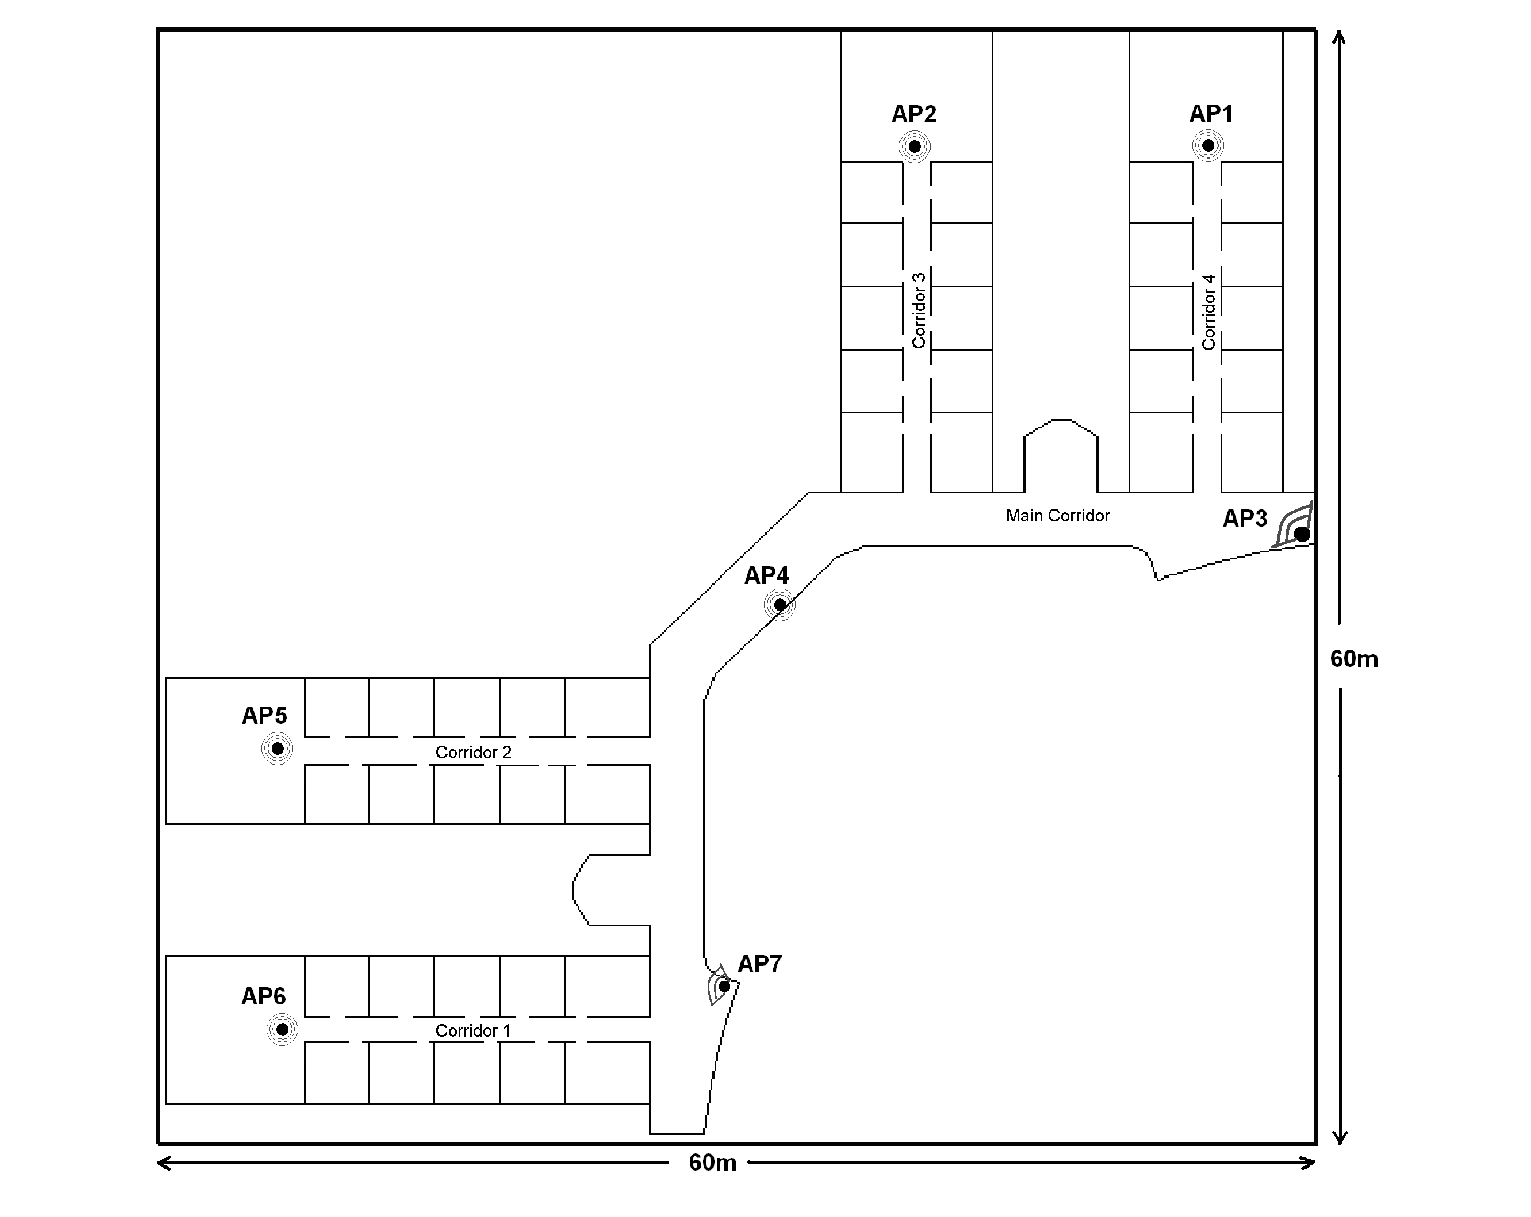
\includegraphics[width=4.7in]{Figure1}
  % where an .eps filename suffix will be assumed under latex, and a .pdf suffix will be assumed for pdflatex
  \caption{Departamento de Electrónica.}
  \label{fig:fig1}
\end{figure}

Y ahora un ejemplo en el que ponemos el \texttt{caption} en el lateral:

\begin{SCfigure}
  \centering 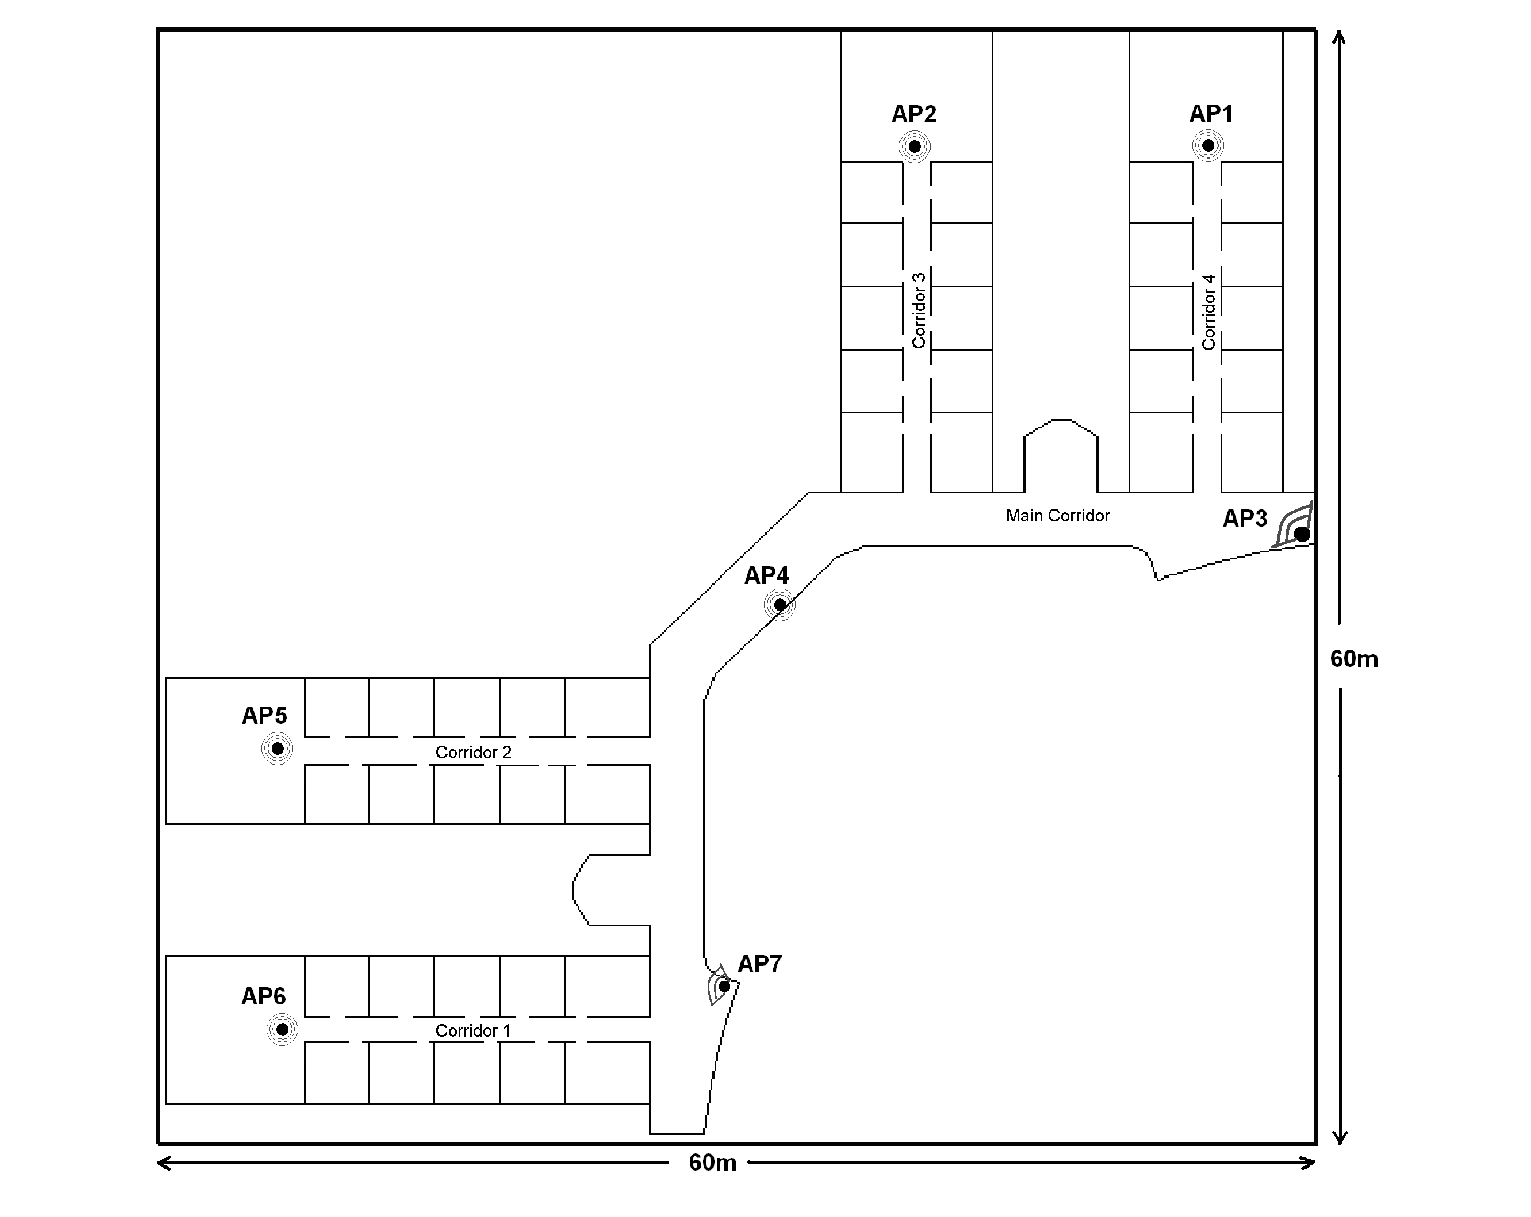
\includegraphics[width=0.5\textwidth]{Figure1}
  \caption{Departamento de Electrónica en el lateral.}
\end{SCfigure}



\section{Técnicas utilizadas}
\label{sec:tecnicas-utilizadas}

Aquí vamos a probar todos los niveles de sección disponibles, para evaluar la asignación de \texttt{tocdepth}...

Blah, blah, blah\ldots


\subsection{Subsección}
\label{sec:subseccion}


\subsubsection{Subsubsección}
\label{sec:subsubseccion}

\paragraph{Paragraph}
\label{sec:paragraph-1}


\subparagraph{Subparagraph}
\label{sec:subparagraph}



\section{Conclusiones}
\label{sec:conclusiones-teoria}

Blah, blah, blah\ldots

%%% Local Variables:
%%% TeX-master: "../book"
%%% End:


%%%%%%%%%%%%%%%%%%%%%%%%%%%%%%%%%%%%%%%%%%%%%%%%%%%%%%%%%%%%%%%%%%%%%%%%%%%
%
% Generic template for TFC/TFM/TFG/Tesis
%
% $Id: desarrollo.tex,v 1.1 2015/06/05 00:05:19 macias Exp $
%
% By:
%  + Javier Macías-Guarasa. 
%    Departamento de Electrónica
%    Universidad de Alcalá
%  + Roberto Barra-Chicote. 
%    Departamento de Ingeniería Electrónica
%    Universidad Politécnica de Madrid   
% 
% Based on original sources by Roberto Barra, Manuel Ocaña, Jesús Nuevo,
% Pedro Revenga, Fernando Herránz and Noelia Hernández. Thanks a lot to
% all of them, and to the many anonymous contributors found (thanks to
% google) that provided help in setting all this up.
%
% See also the additionalContributors.txt file to check the name of
% additional contributors to this work.
%
% If you think you can add pieces of relevant/useful examples,
% improvements, please contact us at (macias@depeca.uah.es)
%
% You can freely use this template and please contribute with
% comments or suggestions!!!
%
%%%%%%%%%%%%%%%%%%%%%%%%%%%%%%%%%%%%%%%%%%%%%%%%%%%%%%%%%%%%%%%%%%%%%%%%%%%

\chapter{Desarrollo}
\label{cha:development}


\begin{FraseCelebre}
  \begin{Frase}
    A fuerza de construir bien, se llega a buen
    arquitecto\footnote{Tomado de ejemplos del proyecto \texis{}.}.
  \end{Frase}
  \begin{Fuente}
    Aristóteles
  \end{Fuente}
\end{FraseCelebre}



\section{Introducción}
\label{sec:development-introduction}

Blah, blah, blah.

La estructura de este capítulo es\ldots


\section{Sección 1 del capítulo de desarrollo}
\label{sec:development-1}

Blah, blah, blah.


\subsection{Subsección 1.1 del capítulo de desarrollo}
\label{sec:development-11}

Blah, blah, blah.


\subsection{Subsección 1.2 del capítulo de desarrollo}
\label{sec:development-12}

Blah, blah, blah.



\section{Sección 2 del capítulo de desarrollo}
\label{sec:development-2}

Blah, blah, blah.




\section{Conclusiones}
\label{sec:development-conclusions}

Blah, blah, blah.



%%% Local Variables:
%%% TeX-master: "../book"
%%% End:


%%%%%%%%%%%%%%%%%%%%%%%%%%%%%%%%%%%%%%%%%%%%%%%%%%%%%%%%%%%%%%%%%%%%%%%%%%%
%
% Generic template for TFC/TFM/TFG/Tesis
%
% $Id: resultados.tex,v 1.7 2016/03/31 10:44:23 macias Exp $
%
% By:
%  + Javier Macías-Guarasa.
%    Departamento de Electrónica
%    Universidad de Alcalá
%  + Roberto Barra-Chicote.
%    Departamento de Ingeniería Electrónica
%    Universidad Politécnica de Madrid
% 
% Based on original sources by Roberto Barra, Manuel Ocaña, Jesús Nuevo, Pedro Revenga, Fernando Herránz and Noelia Hernández. Thanks a lot to all of them, and to the many anonymous contributors found (thanks to google) that provided help in setting all this up.
%
% See also the additionalContributors.txt file to check the name of additional contributors to this work.
%
% If you think you can add pieces of relevant/useful examples, improvements, please contact us at (macias@depeca.uah.es)
%
% You can freely use this template and please contribute with comments or suggestions!!!
%
%%%%%%%%%%%%%%%%%%%%%%%%%%%%%%%%%%%%%%%%%%%%%%%%%%%%%%%%%%%%%%%%%%%%%%%%%%%

\chapter{Resultados}
\label{cha:resultados}


\begin{FraseCelebre}
  \begin{Frase}
    % Si quieres ser leído más de una vez, no vaciles en borrar a menudo.
    Rem tene, verba sequentur (Si dominas el tema, las palabras vendrán solas)\footnote{Tomado de ejemplos del proyecto \texis{}.}.
  \end{Frase}
  \begin{Fuente}
    % Horacio
    Catón el Viejo
  \end{Fuente}
\end{FraseCelebre}

\section{Introducción}
\label{sec:introduccion-resultados}

En este capítulo se introducirán los resultados más relevantes del trabajo.

La estructura del capítulo es\ldots


\section{Entorno experimental}
\label{sec:entorno-experimental}

Blah, blah, blah.


\subsection{Bases de datos utilizadas}
\label{sec:bases-de-datos-1}

Blah, blah, blah.


\subsection{Métricas de calidad}
\label{sec:metricas-de-calidad}

Blah, blah, blah.

En la tabla\ref{pruebaCalc2LaTeX} pongo un ejemplo del uso del conversor de libreoffice a \LaTeX{} (cortesía de Roberto Chamorro). Para usarlo tienes que importar la macro que encontrarás en el directorio \texttt{Tools/calc2latex//calc2latex\_024\_eur\_latex}\footnote{Para ello sigue el proceso de importación que se describe en \url{http://ask.libreoffice.org/en/question/35598/where-are-lo-basic-macros-stored/}, importando Cals y cuando ejecutes la macro hazlo por el punto de entrada \texttt{Main}, después de seleccionar el rango de celdas de la tabla.}

\begin{table}[htbp]
\caption{Caption de prueba de tabla LaTeX convertida desde
  \texttt{libreoffice} con la macro \texttt{calc2latex}.}
\begin{center}
\begin{tabular}{|l|r|r|r|}
\hline
 & \multicolumn{1}{l|}{System A} & \multicolumn{1}{l|}{System B} & \multicolumn{1}{l|}{System C} \\ \hline
FA rate & 10,00\% & 5,00\% & 2,00\% \\ \hline
TA rate & 90,00\% & 85,00\% & 75,00\% \\ \hline
\end{tabular}
\end{center}
\label{pruebaCalc2LaTeX}
\end{table}




\subsection{Estrategia y metodología de experimentación}
\label{sec:estr-y-metod}

Blah, blah, blah.


\section{Resultados experimentales}
\label{sec:result-experim}

A continuación, se muestra un ejemplo de tabla simple (ver tabla \ref{tab:table1}).

\begin{table}
  % increase table row spacing, adjust to taste
  \renewcommand{\arraystretch}{1.3}
  \caption{Comparativa.}
  \label{tab:table1}
  \begin{center}
    % Some packages, such as MDW tools, offer better commands for making tables than the plain LaTeX2e tabular which is used here.
    \begin{tabular}{|c|c|c|}
      \hline
      Method & Training Time & Man-Work (\%)\\
      \hline
      Propagation model & $<$ 30 sec & 5\\
      \hline
      Manual & 9 h 30 min & 24\\
      \hline
      Automatic & 2 h & 10 8\\
      \hline
    \end{tabular}
  \end{center}
\end{table}

Cuando las tablas ocupan más de un página se debe utilizar un tipo especial de tablas denominado \texttt{longtable}. A continuación, se muestra un ejemplo del mismo (ver tabla \ref{table2}).

\begin{center}
	\begin{longtable}{|c|c|c|c|}
    \caption[Resultados de la correlación cruzada.]{Resultados de la correlación cruzada.} \label{table2} \\
    
    \hline \multicolumn{1}{|c|}{\textbf{Posición Real}} & \multicolumn{1}{c|}{\textbf{Posición estimada}} & \multicolumn{1}{c|}{\textbf{Coef. Correlación}} & \multicolumn{1}{c|}{\textbf{Acierto/Fallo}} \\ \hline 
    \endfirsthead
    
    \multicolumn{4}{c}%
    {{\bfseries \tablename\ \thetable{} -- continúa en la página anterior}} \\
    \hline \multicolumn{1}{|c|}{\textbf{Posición Real}} & \multicolumn{1}{c|}{\textbf{Posición estimada}} & \multicolumn{1}{c|}{\textbf{Coef. Correlación}} & \multicolumn{1}{c|}{\textbf{Acierto/Fallo}} \\ \hline 
    \endhead
    
    \hline \multicolumn{4}{|r|}{{Continúa en la página siguiente}} \\ \hline
    \endfoot

    \hline \hline
    \endlastfoot
    
    \hline	2P0	&	2P0	&	0,004954	&	A	\\
    \hline	2P1	&	2P4	&	0,005752	&	F	\\
    \hline	2P2	&	2P2	&	0,005461	&	A	\\
    \hline	2P3	&	2P0	&	0,004634	&	F	\\
    \hline	2P5	&	2P4	&	0,005991	&	F	\\
    \hline	2P6	&	2P16	&	0,004410	&	F	\\
    \hline	2P7	&	3P9	&	0,008038	&	F	\\
    \hline	2P8	&	3P9	&	0,003753	&	F	\\
    \hline	2P9	&	2P7	&	0,004908	&	F	\\
    \hline	2P10	&	2P10	&	0,007273	&	A	\\
    \hline	2P14	&	2P16	&	0,006485	&	F	\\
    \hline	2P15	&	2P15	&	0,004932	&	A	\\
    \hline	2P16	&	2P16	&	0,006237	&	A	\\
    \hline	2P17	&	2P15	&	0,005110	&	F	\\
    \hline	2P18	&	3P18	&	0,006235	&	F	\\
    \hline	2P19	&	3P18	&	0,004827	&	F	\\
    \hline	2P20	&	2P20	&	0,006877	&	A	\\
    \hline	2P22	&	3P18	&	0,003048	&	F	\\
    \hline	2P24	&	2P24	&	0,006833	&	A	\\
    \hline	2P25	&	2P25	&	0,004875	&	A	\\
    \hline	2P26	&	2P31	&	0,005511	&	F	\\
    \hline	2P27	&	2P28	&	0,004590	&	F	\\
    \hline	2P30	&	2P31	&	0,005576	&	F	\\
    \hline	2P31	&	2P31	&	0,007213	&	A	\\
    \hline	2P32	&	2P35	&	0,003340	&	F	\\
    \hline	2P34	&	2P34	&	0,004128	&	A	\\
    \hline	2P36	&	2P35	&	0,003329	&	F	\\
    \hline	2P37	&	2P37	&	0,003468	&	A	\\
    \hline	2P39	&	2P38	&	0,002577	&	F	\\
    \hline	2P40	&	2P43	&	0,004303	&	F	\\
    \hline	2P41	&	2P41	&	0,001573	&	A	\\
    \hline	2P42	&	2P41	&	0,000846	&	F	\\
    \hline	2P44	&	2P44	&	0,002732	&	A	\\
    \hline	2P45	&	23P45	&	0,001958	&	F	\\
    \hline	2P47	&	2P34	&	0,002869	&	F	\\
    \hline	2P48	&	2P43	&	0,004569	&	F	\\
    \hline	2P49	&	3P51	&	0,001374	&	F	\\
    \hline	2P50	&	2P34	&	0,002274	&	F	\\
    \hline	2P51	&	2P63	&	0,003931	&	F	\\
    \hline	2P52	&	2P55	&	0,003537	&	F	\\
    \hline	2P53	&	3P56	&	0,003126	&	F	\\
    \hline	2P54	&	2P67	&	0,005560	&	F	\\
    \hline	2P56	&	2P55	&	0,002817	&	F	\\
    \hline	2P57	&	2P67	&	0,006168	&	F	\\
    \hline	2P58	&	2P58	&	0,005278	&	A	\\
    \hline	2P60	&	3P66	&	0,004966	&	F	\\
    \hline	2P61	&	3P61	&	0,004748	&	A	\\
    \hline	2P64	&	2P67	&	0,005342	&	F	\\
    \hline	2P66	&	2P4	&	0,004172	&	F	\\
    \hline	2P67	&	2P67	&	0,005706	&	A	\\
    \hline	3P0	&	3P0	&	0,003674	&	A	\\
    \hline	3P61	&	2P61	&	0,003263	&	F	\\
    \hline	3P64	&	2P67	&	0,003484	&	F	\\
    \hline	3P65	&	2P67	&	0,002975	&	F	\\
    \hline	3P66	&	2P58	&	0,005029	&	F	\\
    \hline	3P67	&	3P67	&	0,003714	&	A	\\
	\end{longtable}
\end{center}

En algunas ocasiones, también resulta útil emplear el entorno
\texttt{subfigure} para añadir múltiples imágenes dentro de la misma
figura. A continuación, se muestra un ejemplo del uso en la figura
\ref{fig:fig3}. También se pueden referenciar las sub-figuras de forma
individual, por ejemplo la sub-figura \ref{fig:fig3b} (usando un método
de cita), o bien la sub-figura \ref{fig:fig3}.\subref{fig:fig3b} (usando
otro alternativo).

% For this to work you need to (in preamble.tex):
% - remove \usepackage{subfig}
% - add \usepackage{caption}
% - add \usepackage{subcaption}
\begin{figure}
  \centering
  \begin{subfigure}[b]{0.3\textwidth}
    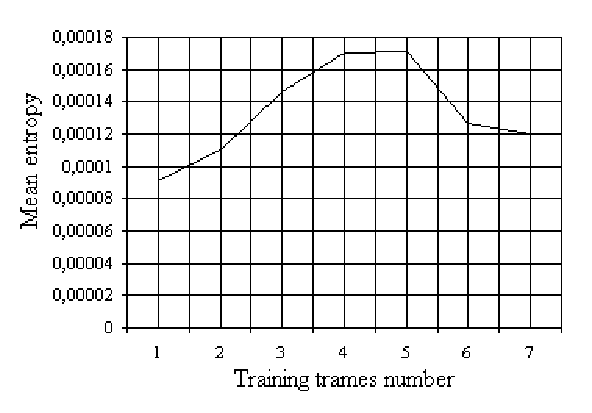
\includegraphics[width=\textwidth]{Figure2}
    \caption{Mean Entropy.}
    \label{fig:fig3a}
  \end{subfigure}%
  ~ %add desired spacing between images, e. g. ~, \quad, \qquad etc.
  % (or a blank line to force the subfigure onto a new line)
  \begin{subfigure}[b]{0.3\textwidth}
    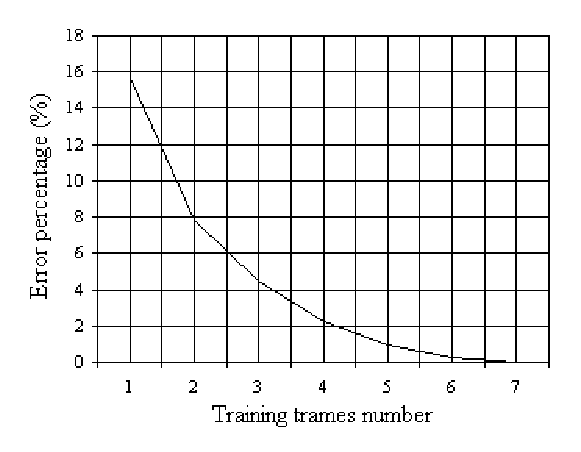
\includegraphics[width=\textwidth]{Figure3}
    \caption{Error Percentage.}
    \label{fig:fig3b}
  \end{subfigure}
  \caption{Optimal trames number in the training data set.}
  \label{fig:fig3}
\end{figure}

La figura~\ref{fig:LIdiapRoom} muestra otro ejemplo con referencias a las subfigures en el caption principal.

\begin{figure}
  \centering
  \begin{subfigure}[b]{0.30\textwidth}
    
\includegraphics[width=\textwidth]{roomlayout2}
    \caption{}
    \label{fig:RoomLayout}
  \end{subfigure}%
  \qquad \qquad %add desired spacing between images, e. g. ~, \quad, \qquad, \hfill etc.
  % (or a blank line to force the subfigure onto a new line)
  \begin{subfigure}[b]{0.425\textwidth}
    \includegraphics[width=\textwidth]{idiap-seq45-cam2.jpg}
    \caption{}
    \label{fig:RoomPicture}
  \end{subfigure}
  \caption{Idiap Smart Meeting Room for AV16.3 recordings. (\protect\subref{fig:RoomLayout}) Room layout showing the centered table, and the microphones arranged in two circular arrays. (\protect\subref{fig:RoomPicture}) Sample of recorded video frame showing the arrays area. \vspace{-0.3cm}}
  \label{fig:LIdiapRoom}
\end{figure}

Os incluimos a continuación un párrafo de un artículo en el que hacemos referencia a varias figuras y subfiguras:

\emph{The IDIAP Meeting Room (shown in figure~\ref{fig:LIdiapRoom}) is a $8.2m \times 3.6m \times 2.4m$ rectangular space containing a centrally located $4.8m \times 1.2m$ rectangular table, on top of which two circular microphone arrays of $10 cm$ radius are located, each of them composed by 8 microphones. The centers of the two arrays are separated by $80 cm$ and the origin of coordinates is located in the middle point between the two arrays. The arrays can be also seen in figures~\ref{fig:simureal_positions}.\subref{fig:Simulated_positions}, ~\ref{fig:simureal_positions}.\subref{fig:real_positions_short}, and ~\ref{fig:simureal_positions}.\subref{fig:real_positions_long}, in which only the relevant section of the room is displayed, each one showing different scenarios that were used in the experiments. A detailed description of the meeting room can be found in~\cite{moore2002}.}

\begin{figure}
  \centering
  \begin{subfigure}[t]{0.3\textwidth}
    
\includegraphics[width=\textwidth]{angular2-short-improved}
    \caption{For validation\\with simulated data.}
    \label{fig:Simulated_positions}
  \end{subfigure}
~%add desired spacing between images, e. g. ~, \quad, \qquad,
  % \hfill etc.
  % (or a blank line to force the subfigure onto a new line)
  \begin{subfigure}[t]{0.3\textwidth}
    
\includegraphics[width=\textwidth]{positions1-short-improved}
    \caption{For validation\\with real data and microphone pairs with $20~cm$ spacing.}
    \label{fig:real_positions_short}
  \end{subfigure}
  ~
  \begin{subfigure}[t]{0.3\textwidth}
    
\includegraphics[width=\textwidth]{positions2-short-improved}
    \caption{For validation\\with real data and microphone pairs with
      $82.46~cm$ spacing.}
    \label{fig:real_positions_long}
  \end{subfigure}
  \caption{Geometrical details for the experiments carried out. Only the
    relevant section of the room is shown, and microphone pairs are
    connected by solid lines.}
  \label{fig:simureal_positions}
\end{figure}

En la figura~\ref{fig:Sim_angles} mostramos un ejemplo de varias
figuras organizadas de forma un poco más complejo.

\begin{figure}
  \centering
  \begin{subfigure}[b]{0.3\textwidth}
    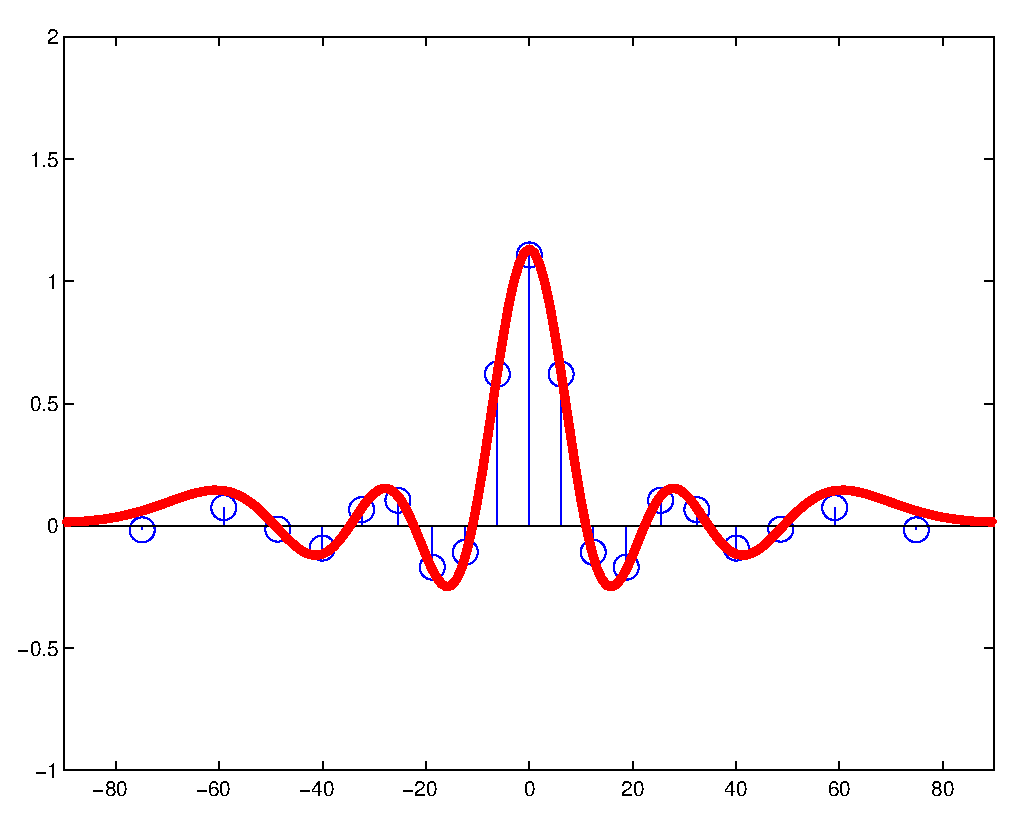
\includegraphics[width=\textwidth]{Sim_seg025_ang090}
    \caption{$0^{\circ}$}
    \label{fig:Sim_ang090}
  \end{subfigure}
  % add desired spacing between images, e. g. ~, \quad, \qquad etc.
  % (or a blank line to force the subfigure onto a new line)

  \begin{subfigure}[b]{0.3\textwidth}
    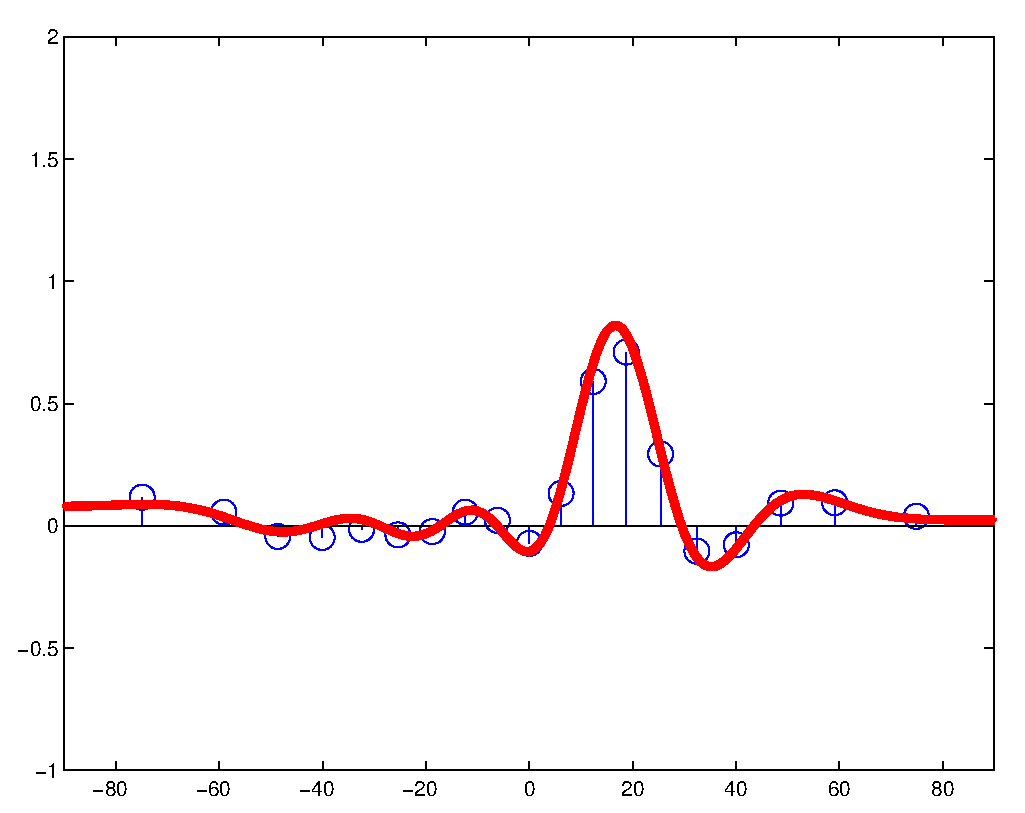
\includegraphics[width=\textwidth]{Sim_seg025_ang108}
    \caption{$18^{\circ}$}
    \label{fig:Sim_ang108}
  \end{subfigure}
  % add desired spacing between images, e. g. ~, \quad, \qquad etc.
  % (or a blank line to force the subfigure onto a new line)
  \begin{subfigure}[b]{0.3\textwidth}
    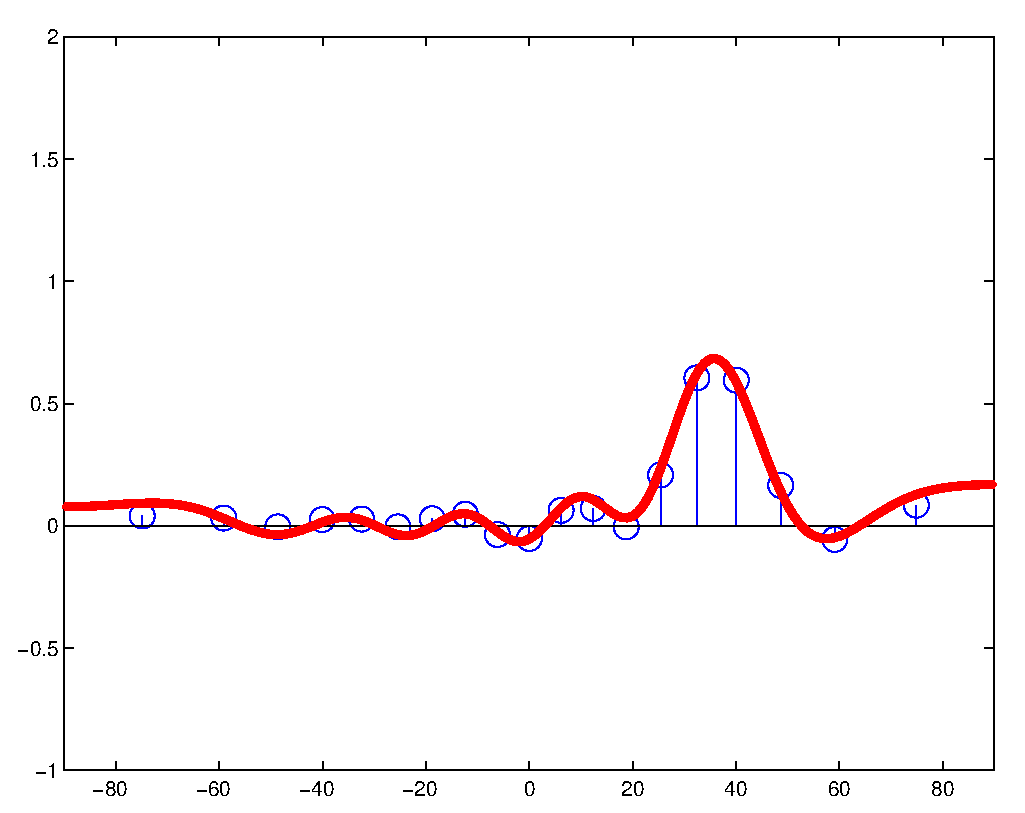
\includegraphics[width=\textwidth]{Sim_seg025_ang126}
    \caption{$36^{\circ}$}
    \label{fig:Sim_ang126}
  \end{subfigure}
  % add desired spacing between images, e. g. ~, \quad, \qquad etc.
  % (or a blank line to force the subfigure onto a new line)
  \begin{subfigure}[b]{0.3\textwidth}
    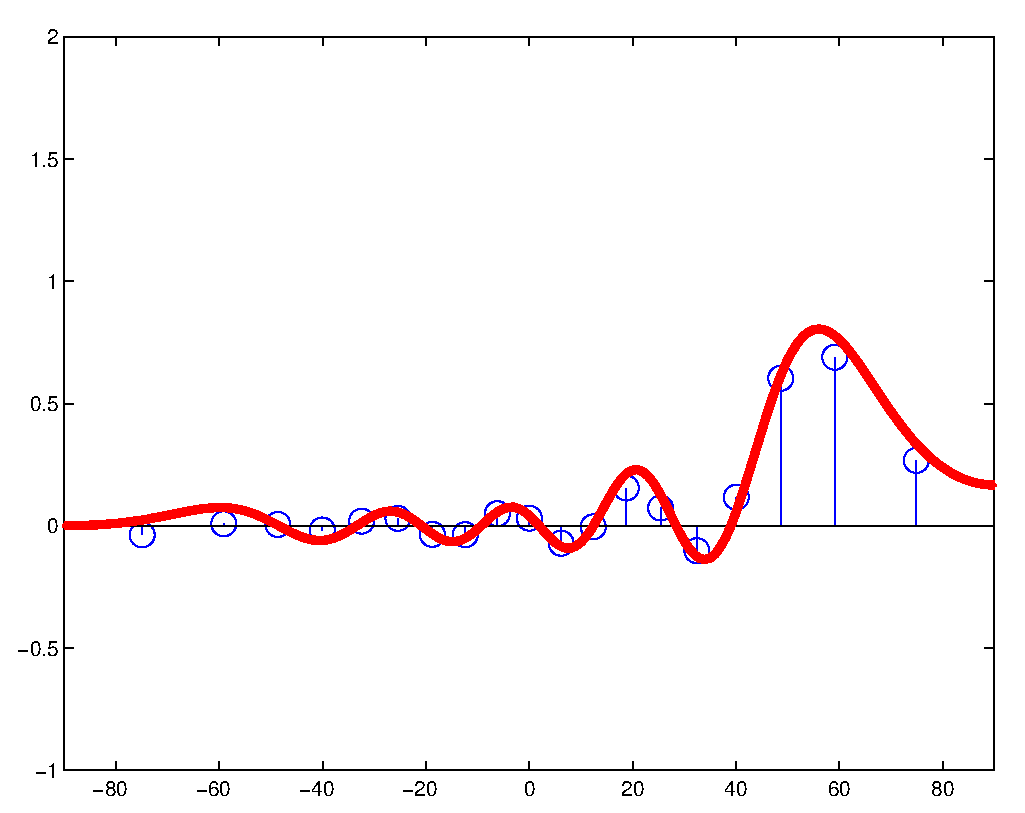
\includegraphics[width=\textwidth]{Sim_seg025_ang144}
    \caption{$54^{\circ}$}
    \label{fig:Sim_ang144}
  \end{subfigure}
  % add desired spacing between images, e. g. ~, \quad, \qquad etc.
  % (or a blank line to force the subfigure onto a new line)

  \begin{subfigure}[b]{0.3\textwidth}
    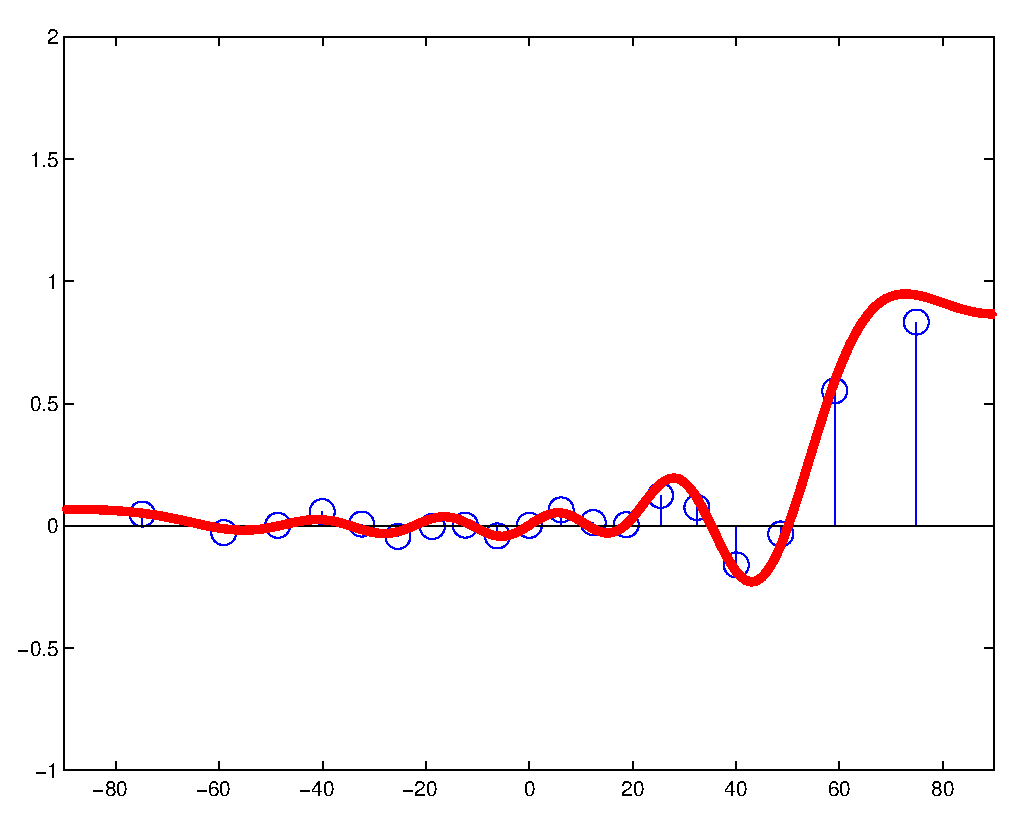
\includegraphics[width=\textwidth]{Sim_seg025_ang162}
    \caption{$72^{\circ}$}
    \label{fig:Sim_ang162}
  \end{subfigure}

  \caption{Comparison between the steered power response generated by the model (solid line) and that calculated using simulated waveforms in the AV16.3 environment (stems). Results for the speaker in given angles and the array steered from -90º to +90º are shown.}
  \label{fig:Sim_angles}
\end{figure}

También es posible incluir el código de una figura en un fichero \texttt{.tex} independiente (para hacer más legible el código del documento principal). Un ejemplo lo tenéis a continuación, incluyendo el texto en inglés del documento original:

\emph{Figure~\ref{fig:SRPvsPatternSelected} includes the results of the comparison, for several speaker positions (1, 2, 4, 6, 8 and 16, emphasized in figure~\ref{fig:simureal_positions}.\subref{fig:real_positions_short}), and selected to provide different acoustic situations, both in terms of distance and angular position with respect to the arrays. All the graphics show the acoustic power map (predicted or calculated) for a regular two-dimensional grid of $10~cm$. The plot is provided from a top view of the room, spanning the full plan at a height of $61~cm$ above the microphone arrays (this height was the ground truth one for sequence 01). For each speaker position shown, three graphics are plotted:}

\begin{itemize}
  \item \emph{The graphics on the left show the SRP-PHAT acoustic power maps generated by the proposed model (for example, the left graphic in figure~\ref{fig:SRPvsPatternSelected}.\subref{fig:SRPvsModel_Fo1500_position1} for position 1).}
  \item \emph{The graphics in the middle show the real SRP-PHAT acoustic power maps calculated using the real acoustic waveforms (for example, the middle graphic in figure~\ref{fig:SRPvsPatternSelected}.\subref{fig:SRPvsModel_Fo1500_position1} for position 1), for a single selected frame.}
  \item \emph{The graphics on the right show the average real SRP-PHAT acoustic power maps, averaging for all the frames in which the user was in the given position (for example, the right graphic in figure~\ref{fig:SRPvsPatternSelected}.\subref{fig:SRPvsModel_Fo1500_position1} for position 1).}
\end{itemize}

\emph{The green point represents the real (ground truth) speaker position, and the black dots represent the positions of the four microphones used. The hyperbolic shapes found in the figure are consistent with the fact that the place of points with equal acoustic power value, for a given microphone pair, is a hyperbola (in our two-dimensional case, being a hyperboloid of revolution in the three-dimensional case).}

\emph{From figure~\ref{fig:SRPvsPatternSelected}, it can clearly be seen that, again, the predictions closely match the results with real data for the different acoustic conditions, even when the simulations are using fixed and frequency independent average reflection coefficients, and that the acoustic model is based on the simplistic image method model.}

\begin{figure}
  \centering
  \begin{subfigure}[t]{0.47\textwidth}
    \begin{minipage}[t]{\textwidth}
      \begin{subfigure}[t]{0.3\textwidth}
        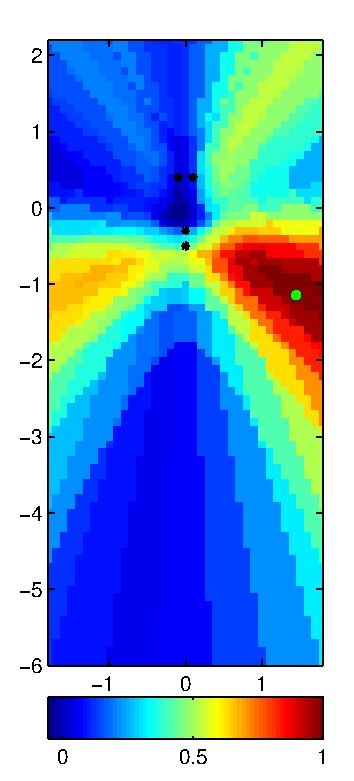
\includegraphics[width=\textwidth]{Pattern_Fo1500_pos01}
        %\caption{SRP Model for pos. 1}
        \label{fig:Pattern_Fo1500_pos01}
      \end{subfigure}
      % ~ %add desired spacing between images, e. g. ~, \quad, \qquad,
      % \hfill etc.
      % (or a blank line to force the subfigure onto a new line)
      \begin{subfigure}[t]{0.3\textwidth}
        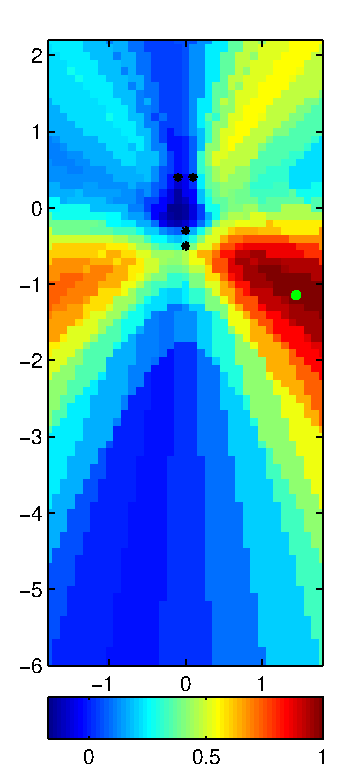
\includegraphics[width=\textwidth]{SRP_Fo1500_frame003_pos01}
        % \caption{Real SRP for pos.  1}
        \label{fig:SRP_Fo1500_pos01}
      \end{subfigure}
      % ~ %add desired spacing between images, e. g. ~, \quad, \qquad,
      % \hfill etc.
      % (or a blank line to force the subfigure onto a new line)
      \begin{subfigure}[t]{0.3\textwidth}
        \includegraphics[width=\textwidth]{SRP_Fo1500_mean_pos01}
        % \caption{Avg. SRP for pos. 1}
        \label{fig:SRP_Fo1500_mean_pos01}
      \end{subfigure}
      \vspace{\verticalSpacingSRPMaps}
      \caption{\centering For position 1}
      \label{fig:SRPvsModel_Fo1500_position1}
      \vspace{0.25cm}
    \end{minipage}
  \end{subfigure}
  ~% \quad % between 1 and 2 %add desired spacing between images, e. g. ~, \quad, \qquad,
  % \hfill etc.
  % (or a blank line to force the subfigure onto a new line)
  \begin{subfigure}[t]{0.47\textwidth}
    \begin{minipage}[t]{\textwidth}
      \begin{subfigure}[t]{0.3\textwidth}
        \includegraphics[width=\textwidth]{Pattern_Fo1500_pos02}
        % \caption{SRP Model for pos. 2}
        \label{fig:Pattern_Fo1500_pos02}
      \end{subfigure}
      % ~ %add desired spacing between images, e. g. ~, \quad, \qquad,
      % \hfill etc.
      % (or a blank line to force the subfigure onto a new line)
      \begin{subfigure}[t]{0.3\textwidth}
        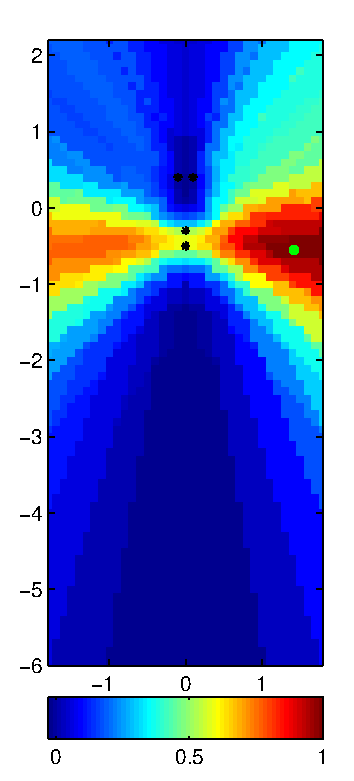
\includegraphics[width=\textwidth]{SRP_Fo1500_frame161_pos02}
        % \caption{Real SRP for pos.  2\\}
        \label{fig:SRP_pos02}
      \end{subfigure}
      % ~ %add desired spacing between images, e. g. ~, \quad, \qquad,
      % \hfill etc.
      % (or a blank line to force the subfigure onto a new line)
      \begin{subfigure}[t]{0.3\textwidth}
        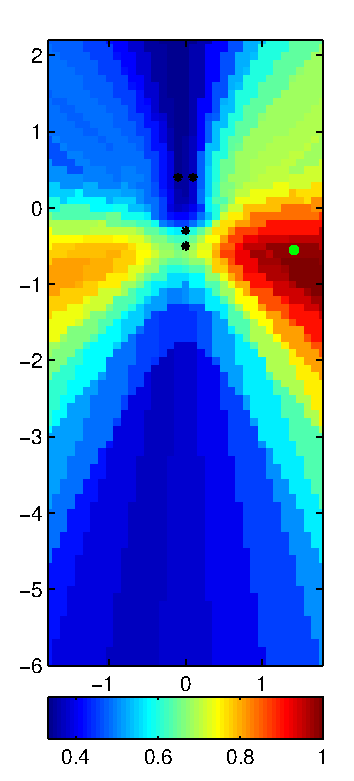
\includegraphics[width=\textwidth]{SRP_Fo1500_mean_pos02}
        % \caption{Avg. SRP for pos. 2}
        \label{fig:SRP_Fo1500_mean_pos02}
      \end{subfigure}
      \vspace{\verticalSpacingSRPMaps}
      \caption{\centering For position 2}
      \vspace{0.25cm}
    \end{minipage}
  \end{subfigure}

  \begin{subfigure}[t]{0.47\textwidth}
    \begin{minipage}[t]{\textwidth}
      \begin{subfigure}[t]{0.3\textwidth}
        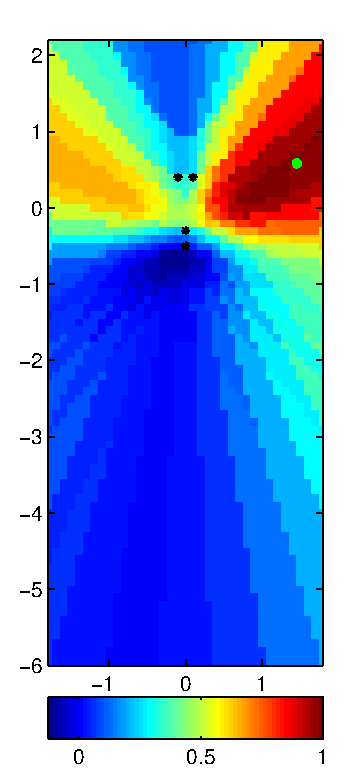
\includegraphics[width=\textwidth]{Pattern_Fo1500_pos04}
        % \caption{SRP Model for pos. 4}
        \label{fig:Pattern_Fo1500_pos04}
      \end{subfigure}
      % ~ %add desired spacing between images, e. g. ~, \quad, \qquad,
      % \hfill etc.
      % (or a blank line to force the subfigure onto a new line)
      \begin{subfigure}[t]{0.3\textwidth}
        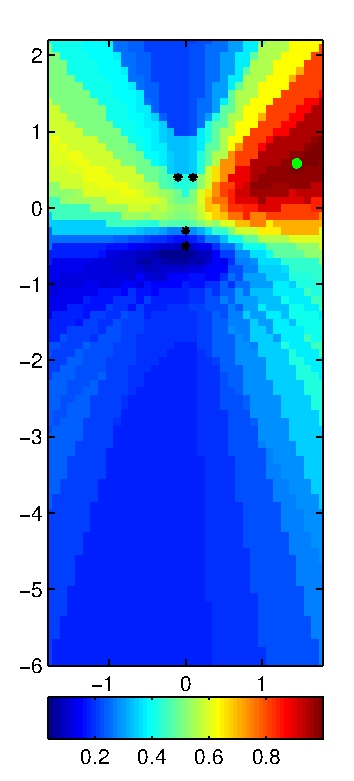
\includegraphics[width=\textwidth]{SRP_Fo1500_frame464_pos04}
        % \caption{Real SRP for pos.  4\\}
        \label{fig:SRP_pos04}
      \end{subfigure}
      % ~ %add desired spacing between images, e. g. ~, \quad, \qquad,
      % \hfill etc.
      % (or a blank line to force the subfigure onto a new line)
      \begin{subfigure}[t]{0.3\textwidth}
        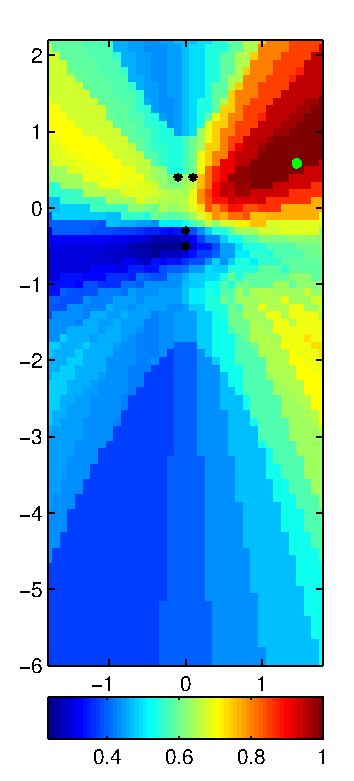
\includegraphics[width=\textwidth]{SRP_Fo1500_mean_pos04}
        % \caption{Avg. SRP for pos. 4}
        \label{fig:SRP_Fo1500_mean_pos04}
      \end{subfigure}
      \vspace{\verticalSpacingSRPMaps}
      \caption{\centering For position 4}
      \vspace{0.25cm}
    \end{minipage}
  \end{subfigure}
  ~%  \qquad % between 4 and 6 %add desired spacing between images, e. g. ~, \quad, \qquad,
  % \hfill etc.
  % (or a blank line to force the subfigure onto a new line)
  \begin{subfigure}[t]{0.47\textwidth}
    \begin{minipage}[t]{\textwidth}
      \begin{subfigure}[t]{0.3\textwidth}
        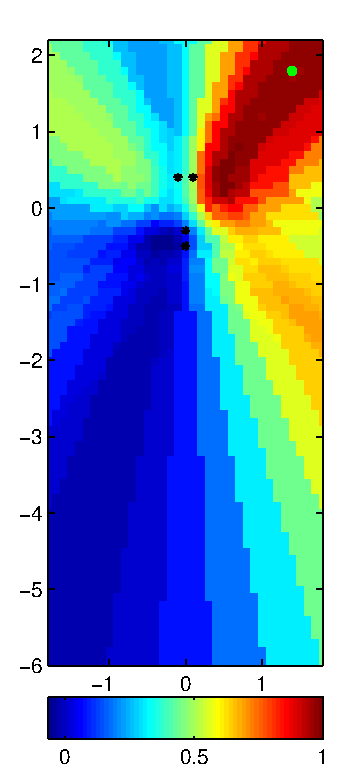
\includegraphics[width=\textwidth]{Pattern_Fo1500_pos06}
        % \caption{SRP Model for pos. 6}
        \label{fig:Pattern_Fo1500_pos06}
      \end{subfigure}
      % ~ %add desired spacing between images, e. g. ~, \quad, \qquad,
      % \hfill etc.
      % (or a blank line to force the subfigure onto a new line)
      \begin{subfigure}[t]{0.3\textwidth}
        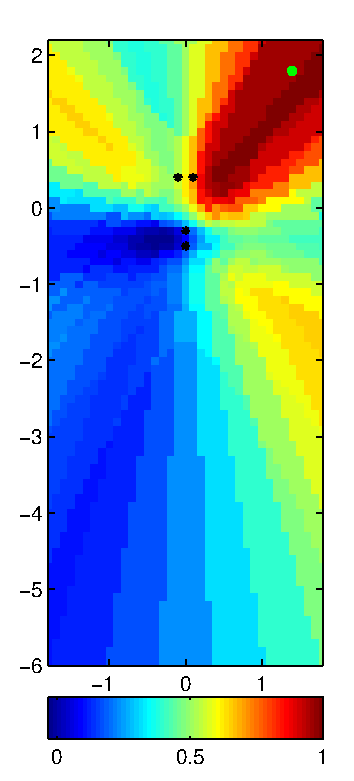
\includegraphics[width=\textwidth]{SRP_Fo1500_frame809_pos06}
        % \caption{Real SRP for pos.  6\\}
        \label{fig:SRP_pos06}
      \end{subfigure}
      % ~ %add desired spacing between images, e. g. ~, \quad, \qquad,
      % \hfill etc.
      % (or a blank line to force the subfigure onto a new line)
      \begin{subfigure}[t]{0.3\textwidth}
        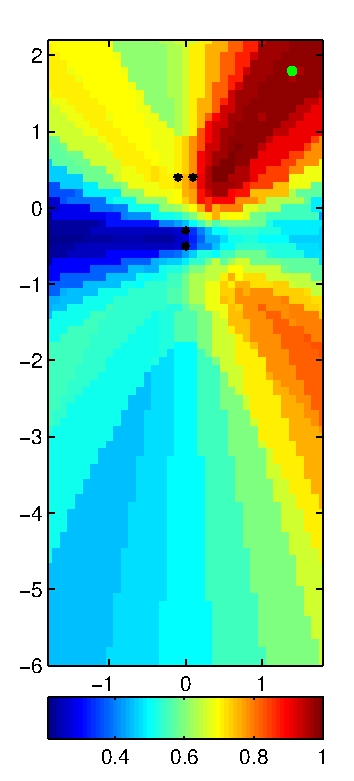
\includegraphics[width=\textwidth]{SRP_Fo1500_mean_pos06}
        % \caption{Avg. SRP for pos. 6}
        \label{fig:SRP_Fo1500_mean_pos06}
      \end{subfigure}
      \vspace{\verticalSpacingSRPMaps}
      \caption{\centering For position 6}
      \vspace{0.25cm}
    \end{minipage}
  \end{subfigure}

  \begin{subfigure}[t]{0.47\textwidth}
    \begin{minipage}[t]{\textwidth}
      \begin{subfigure}[t]{0.3\textwidth}
        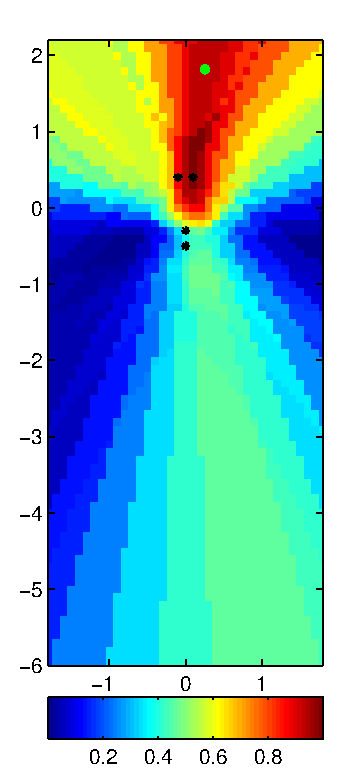
\includegraphics[width=\textwidth]{Pattern_Fo1500_pos08}
        % \caption{SRP Model for pos. 8}
        \label{fig:Pattern_Fo1500_pos08}
      \end{subfigure}
      % ~ %add desired spacing between images, e. g. ~, \quad, \qquad,
      % \hfill etc.
      % (or a blank line to force the subfigure onto a new line)
      \begin{subfigure}[t]{0.3\textwidth}
        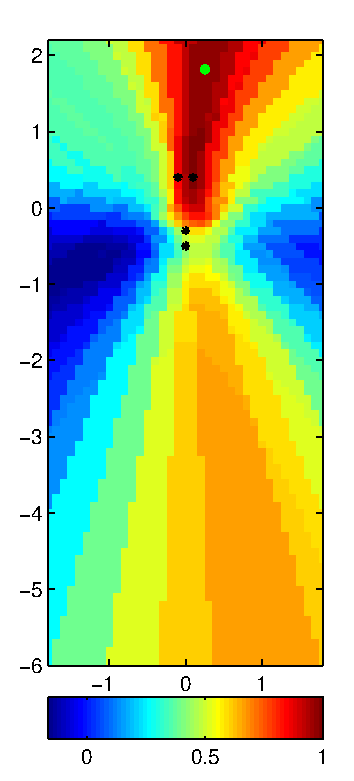
\includegraphics[width=\textwidth]{SRP_Fo1500_frame1127_pos08}
        % \caption{Real SRP for pos.  8\\}
        \label{fig:SRP_pos08}
      \end{subfigure}
      % ~ %add desired spacing between images, e. g. ~, \quad, \qquad,
      % \hfill etc.
      % (or a blank line to force the subfigure onto a new line)
      \begin{subfigure}[t]{0.3\textwidth}
        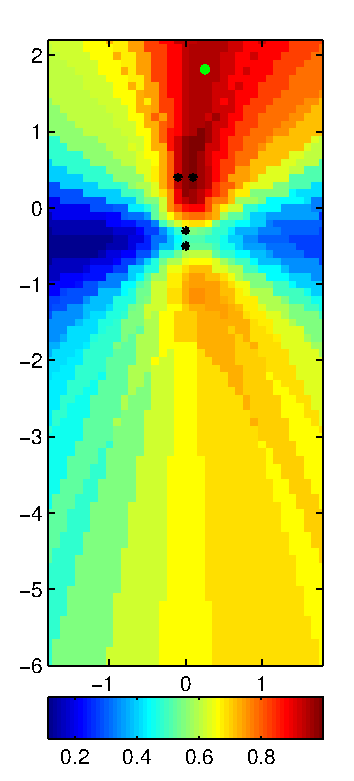
\includegraphics[width=\textwidth]{SRP_Fo1500_mean_pos08}
        % \caption{Avg. SRP for pos. 8}
        \label{fig:SRP_Fo1500_mean_pos08}
      \end{subfigure}
      \vspace{\verticalSpacingSRPMaps}
      \caption{\centering For position 8}
      \vspace{0.25cm}
    \end{minipage}
  \end{subfigure}
  ~%  \qquad % between 8 and 16 %add desired spacing between images, e. g. ~, \quad, \qquad,
  % \hfill etc.
  % (or a blank line to force the subfigure onto a new line)
  \begin{subfigure}[t]{0.47\textwidth}
    \begin{minipage}[t]{\textwidth}
      \begin{subfigure}[t]{0.3\textwidth}
        \includegraphics[width=\textwidth]{Pattern_Fo1500_pos16}
        % \caption{SRP Model for pos. 16}
        \label{fig:Pattern_Fo1500_pos16}
      \end{subfigure}
      % ~ %add desired spacing between images, e. g. ~, \quad, \qquad,
      % \hfill etc.
      % (or a blank line to force the subfigure onto a new line)
      \begin{subfigure}[t]{0.3\textwidth}
        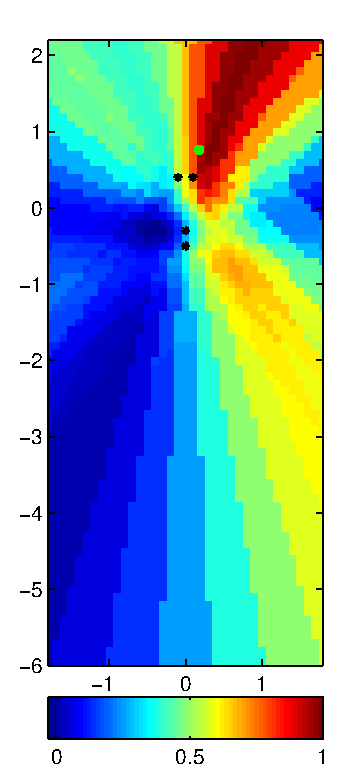
\includegraphics[width=\textwidth]{SRP_Fo1500_frame2518_pos16}
        % \caption{Real SRP for pos. 16\\}
        \label{fig:SRP_pos16}
      \end{subfigure}
      % ~ %add desired spacing between images, e. g. ~, \quad, \qquad,
      % \hfill etc.
      % (or a blank line to force the subfigure onto a new line)
      \begin{subfigure}[t]{0.3\textwidth}
        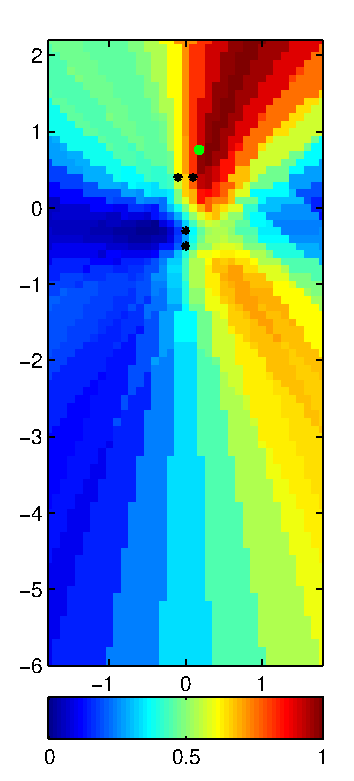
\includegraphics[width=\textwidth]{SRP_Fo1500_mean_pos16}
        % \caption{Avg. SRP for pos. 16}
        \label{fig:SRP_Fo1500_mean_pos16}
      \end{subfigure}
      \vspace{\verticalSpacingSRPMaps}
      \caption{\centering For position 16}
      \vspace{0.25cm}
    \end{minipage}
  \end{subfigure}
  \caption{Comparison between the SRP-PHAT map predicted by the model
    (left graphics),
    the real SRP-PHAT map (middle graphics), and the average (real)
    SRP-PHAT map (right graphics), for
    several speaker positions ($f_0=1.5~KHz$). See
    figure~~\ref{fig:simureal_positions}.\subref{fig:real_positions_short}
    for geometrical references.}
  \label{fig:SRPvsPatternSelected}
\end{figure}
 

\begin{wrapfigure}{r}{0.5\textwidth} 
\vspace{-20pt}
  \begin{center}
    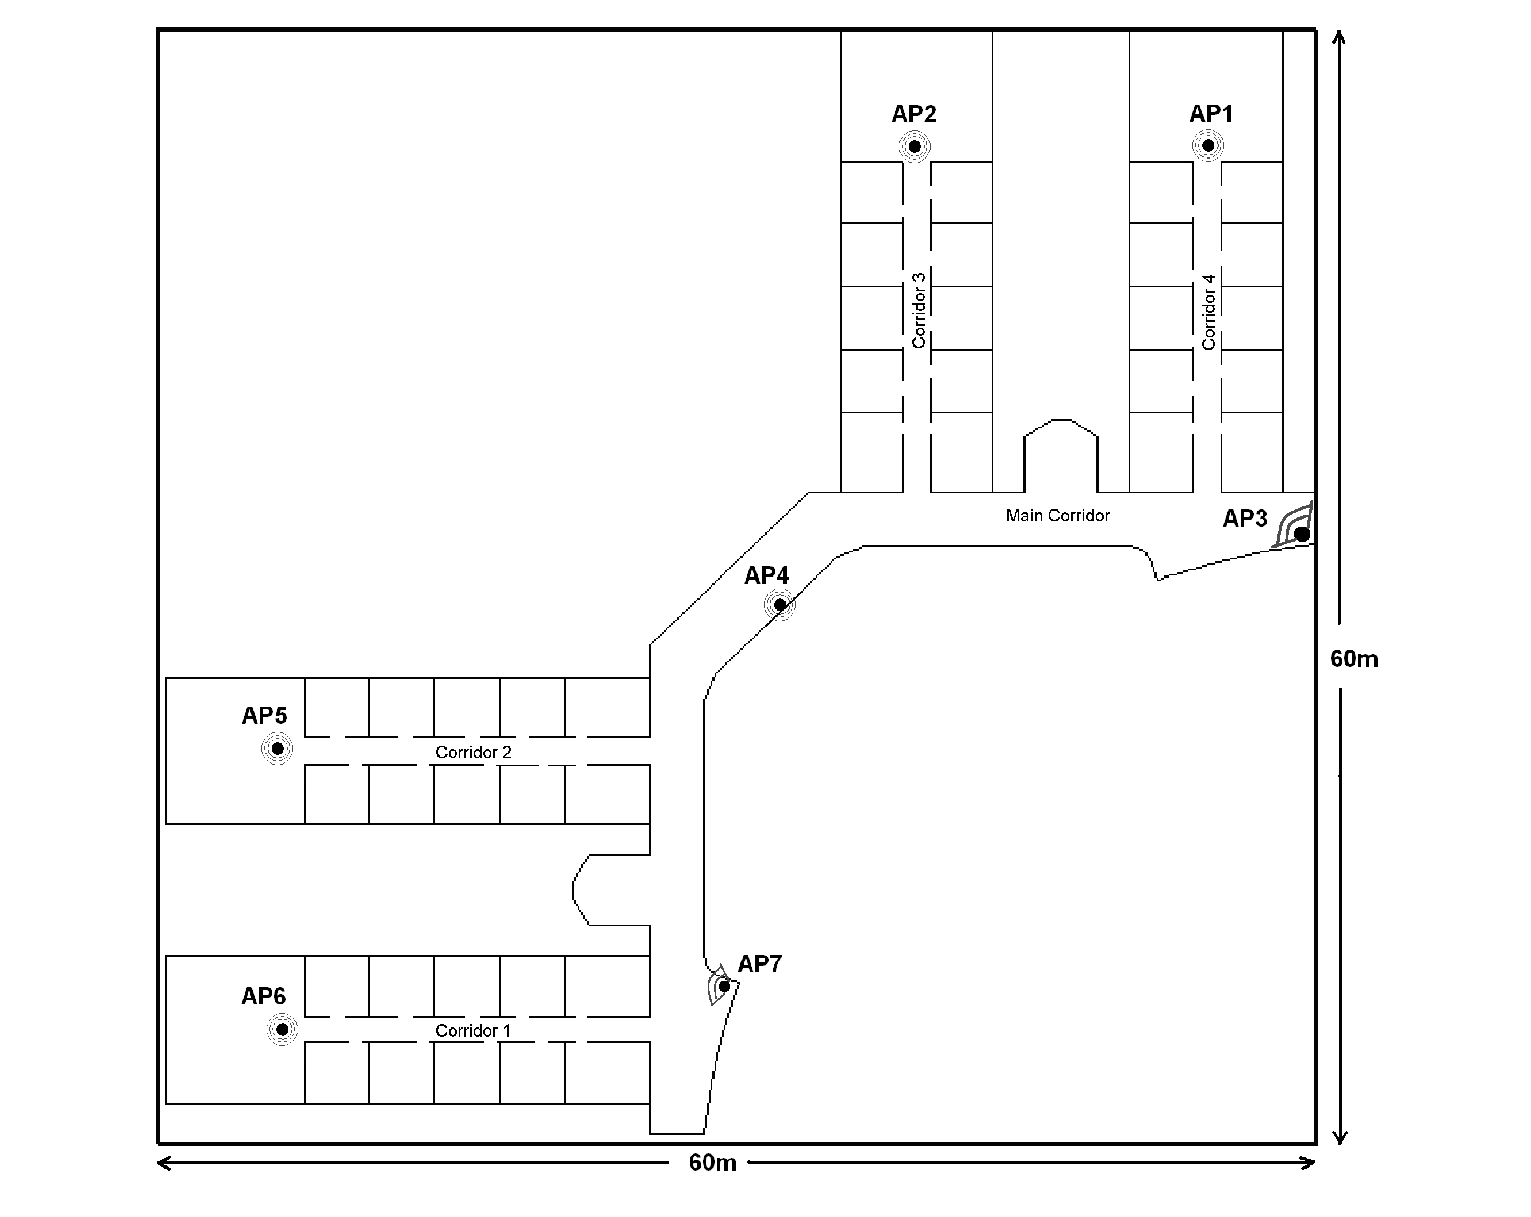
\includegraphics[width=0.4\textwidth]{Figure1}
    \caption{Ejemplo de figura con wrapfigure.}
    \label{fig:wrapfigure1}
  \end{center}
  \vspace{-20pt}
  \vspace{1pt}
\end{wrapfigure} 

Otra posibilidad es utilizar el entorno \texttt{wrapfig} para hacer que el texto bordee a las figuras, como en la figura~\ref{fig:wrapfigure1}. Añado ahora unas líneas de loren ipsum para que lo veáis bien. \lipsum[1-1]

% \lipsum[1-4]
% \begin{wrapfigure}{R}{5cm}
% \centering
% \rule{3cm}{7cm}
% \end{wrapfigure}
% \lipsum[1-6]

Incluso podemos poner una tabla ``apaisada'', como en la \ref{tab:tablas2006}, donde se muestra un resumen de los resultados obtenidos en una serie de experimentos de localización de locutores.

\clearpage
% \begin{table}[H]\centering
\begin{sidewaystable}[hbtp]
  \begin{center}

    \begin{tabular}{||l|c|c|c|c|c||}
      \hline \hline
      & UKA & ITC & AIT & UPC & IBM\\
      \hline
      \hline
      Pcor & $57.0\pm1.4\%$ & $84.0\pm3.3\%$ & $47.0\pm3.1\%$ & $20.0\pm2.5\%$ & $67.0\pm2.9\%$ \\
      \hline
      Bias fine (x:y:z) [mm] & $20:-42:-75$ & $45:27:-41$ & $-27:-77:-40$ & $-59:112:52$ & $91:-69:-38$ \\
      \hline
      Bias fine+gross (x,y,z) [mm] & $735:-93:-258$ & $67:439:-134$ & $17:-402:-118$ & $-141:255:39$ & $474:-141:-14$ \\
      \hline
      AEE fine [mm] = MOTP & $210$ & $130$ & $266$ & $344$ & $228$ \\
      \hline
      Fine+gross [mm] & $1201$ & $632$ & $1006$ & $1188$ & $884$ \\
      \hline
      Loc. frames & $5035$ & $22$ & $995$ & $977$ & $1023$ \\
      \hline
      Ref. duration (s) & $6287.0$ & $596.0$ & $1143.0$ & $1180.0$ & $1194.0$ \\
      \hline \hline
    \end{tabular}
    \caption{Resultados TEST CLEAR 2006.}
    \label{tab:tablas2006}
  \end{center}
\end{sidewaystable}
% \end{table}


\section{Conclusiones}
\label{sec:conclusiones-resultados}

Blah, blah, blah.


%%% Local Variables:
%%% TeX-master: "../book"
%%% End:


%%%%%%%%%%%%%%%%%%%%%%%%%%%%%%%%%%%%%%%%%%%%%%%%%%%%%%%%%%%%%%%%%%%%%%%%%%%
%
% Generic template for TFC/TFM/TFG/Tesis
%
% By:
%  + Javier Macías-Guarasa.
%    Departamento de Electrónica
%    Universidad de Alcalá
%  + Roberto Barra-Chicote.
%    Departamento de Ingeniería Electrónica
%    Universidad Politécnica de Madrid
%
% By: + Javier Macías-Guarasa. Departamento de Electrónica Universidad de Alcalá + Roberto Barra-Chicote. Departamento de Ingeniería Electrónica Universidad Politécnica de Madrid
% 
% Based on original sources by Roberto Barra, Manuel Ocaña, Jesús Nuevo, Pedro Revenga, Fernando Herránz and Noelia Hernández. Thanks a lot to all of them, and to the many anonymous contributors found (thanks to google) that provided help in setting all this up.
%
% See also the additionalContributors.txt file to check the name of additional contributors to this work.
%
% If you think you can add pieces of relevant/useful examples, improvements, please contact us at (macias@depeca.uah.es)
%
% You can freely use this template and please contribute with comments or suggestions!!!
%
%%%%%%%%%%%%%%%%%%%%%%%%%%%%%%%%%%%%%%%%%%%%%%%%%%%%%%%%%%%%%%%%%%%%%%%%%%%

\chapter{Conclusiones y líneas futuras}
\label{cha:concl-y-line}

En este apartado se resumen las conclusiones obtenidas y se proponen futuras líneas de investigación que se deriven del trabajo.

La estructura del capítulo es...


\section{Conclusiones}
\label{sec:conclusiones}

Para añadir una referencia a un autor, se puede utilizar el paquete \texttt{cite}. En el trabajo \cite{armani03}, se muestra un trabajo...

Y podemos usar de nuevo algún acrónimo, como por ejemplo \ac{TDPSOLA}, o uno ya referenciado como \ac{ANN} que cambia cuando lo usas una segunda vez \ac{ANN}.

Veamos finalmente si funciona una cita inline... al paper de Leticia \fullcite{monasterio2022}... (esto substituye la funcionalidad de bibentry...).


\section{Líneas futuras}
\label{sec:lineas-futuras}

Pues eso.


%%% Local Variables:
%%% TeX-master: "../book"
%%% End:




% Optional in PFCs
%%%%%%%%%%%%%%%%%%%%%%%%%%%%%%%%%%%%%%%%%%%%%%%%%%%%%%%%%%%%%%%%%%%%%%%%%%%%
%
% Generic template for TFC/TFM/TFG/Tesis
%
% $Id: pliego.tex,v 1.3 2013/11/25 00:33:32 macias Exp $
%
% By:
%  + Javier Mac�as-Guarasa. 
%    Departamento de Electr�nica
%    Universidad de Alcal�
%  + Roberto Barra-Chicote. 
%    Departamento de Ingenier�a Electr�nica
%    Universidad Polit�cnica de Madrid   
% 
% Based on original sources by Roberto Barra, Manuel Oca�a, Jes�s Nuevo,
% Pedro Revenga, Fernando Herr�nz and Noelia Hern�ndez. Thanks a lot to
% all of them, and to the many anonymous contributors found (thanks to
% google) that provided help in setting all this up.
%
% See also the additionalContributors.txt file to check the name of
% additional contributors to this work.
%
% If you think you can add pieces of relevant/useful examples,
% improvements, please contact us at (macias@depeca.uah.es)
%
% Copyleft 2013
%
%%%%%%%%%%%%%%%%%%%%%%%%%%%%%%%%%%%%%%%%%%%%%%%%%%%%%%%%%%%%%%%%%%%%%%%%%%%

\chapter{Pliego de condiciones}
\label{cha:pliego-de-condiciones}

Blah, blah, blah.

%%% Local Variables:
%%% TeX-master: "../book"
%%% End:


% Optional in PFCs, compulsory in TFGs
%\chapter{Presupuesto}
\label{cha:presupuesto}

Blah, blah, blah.


%
% END Normal chapters. Edit/modify all within this section
%%%%%%%%%%%%%%%%%%%%%%%%%%%%%%%%%%%%%%%%%%%%%%%%%%%%%%%%%%%%%%%%%%%%%%%%%%%
%%%%%%%%%%%%%%%%%%%%%%%%%%%%%%%%%%%%%%%%%%%%%%%%%%%%%%%%%%%%%%%%%%%%%%%%%%%
%%%%%%%%%%%%%%%%%%%%%%%%%%%%%%%%%%%%%%%%%%%%%%%%%%%%%%%%%%%%%%%%%%%%%%%%%%%
%%%%%%%%%%%%%%%%%%%%%%%%%%%%%%%%%%%%%%%%%%%%%%%%%%%%%%%%%%%%%%%%%%%%%%%%%%%
%%%%%%%%%%%%%%%%%%%%%%%%%%%%%%%%%%%%%%%%%%%%%%%%%%%%%%%%%%%%%%%%%%%%%%%%%%%
%%%%%%%%%%%%%%%%%%%%%%%%%%%%%%%%%%%%%%%%%%%%%%%%%%%%%%%%%%%%%%%%%%%%%%%%%%%
%%%%%%%%%%%%%%%%%%%%%%%%%%%%%%%%%%%%%%%%%%%%%%%%%%%%%%%%%%%%%%%%%%%%%%%%%%%


%%%%%%%%%%%%%%%%%%%%%%%%%%%%%%%%%%%%%%%%%%%%%%%%%%%%%%%%%%%%%%%%%%%%%%%%%%%
% Bibliography
%%%%%%%%%%%%%%%%%%%%%%%%%%%%%%%%%%%%%%%%%%%%%%%%%%%%%%%%%%%%%%%%%%%%%%%%%%%
%%%%%%%%%%%%%%%%%%%%%%%%%%%%%%%%%%%%%%%%%%%%%%%%%%%%%%%%%%%%%%%%%%%%%%%%%%%
%
% Generic template for TFC/TFM/TFG/Tesis
%
% $Id: bibliography.tex,v 1.6 2013/11/25 00:33:31 macias Exp $
%
% By:
%  + Javier Mac�as-Guarasa. 
%    Departamento de Electr�nica
%    Universidad de Alcal�
%  + Roberto Barra-Chicote. 
%    Departamento de Ingenier�a Electr�nica
%    Universidad Polit�cnica de Madrid   
% 
% Based on original sources by Roberto Barra, Manuel Oca�a, Jes�s Nuevo,
% Pedro Revenga, Fernando Herr�nz and Noelia Hern�ndez. Thanks a lot to
% all of them, and to the many anonymous contributors found (thanks to
% google) that provided help in setting all this up.
%
% See also the additionalContributors.txt file to check the name of
% additional contributors to this work.
%
% If you think you can add pieces of relevant/useful examples,
% improvements, please contact us at (macias@depeca.uah.es)
%
% Copyleft 2013
%
%%%%%%%%%%%%%%%%%%%%%%%%%%%%%%%%%%%%%%%%%%%%%%%%%%%%%%%%%%%%%%%%%%%%%%%%%%%

%\bibliographystyle{plainnat}
%\bibliographystyle{dinat}
%\bibliographystyle{unsrt}
\bibliographystyle{IEEEtran}
\bibliography{biblio/biblio}


%%% Local Variables:
%%% TeX-master: "../book"
%%% End:


               % EDIT this file if required


%%%%%%%%%%%%%%%%%%%%%%%%%%%%%%%%%%%%%%%%%%%%%%%%%%%%%%%%%%%%%%%%%%%%%%%%%%%
% BEGIN Appendices. Edit/modigy all within this section
%
% I don't recommend it, but if you want to define "parts", use this...
% BEWARE: I didn't write the english dependent code
%\part*{Ap�ndices}
%\label{part:apendices}

\appendix

%%%%%%%%%%%%%%%%%%%%%%%%%%%%%%%%%%%%%%%%%%%%%%%%%%%%%%%%%%%%%%%%%%%%%%%%%%%
%
% Generic template for TFC/TFM/TFG/Tesis
%
% $Id: manual.tex,v 1.3 2013/11/04 23:46:21 macias Exp $
%
% By:
%  + Javier Mac�as-Guarasa. 
%    Departamento de Electr�nica
%    Universidad de Alcal�
%  + Roberto Barra-Chicote. 
%    Departamento de Ingenier�a Electr�nica
%    Universidad Polit�cnica de Madrid   
% 
% Based on original sources by Roberto Barra, Manuel Oca�a, Jes�s Nuevo,
% Pedro Revenga, Fernando Herr�nz and Noelia Hern�ndez. Thanks a lot to
% all of them, and to the many anonymous contributors found (thanks to
% google) that provided help in setting all this up.
%
% If you think you can add pieces of relevant/useful examples,
% improvements, please contact us at (macias@depeca.uah.es)
%
% Copyleft 2013
%
%%%%%%%%%%%%%%%%%%%%%%%%%%%%%%%%%%%%%%%%%%%%%%%%%%%%%%%%%%%%%%%%%%%%%%%%%%%

\chapter{Manual de usuario}
\label{cha:concl-y-line}

\section{Introducci�n}
\label{sec:introapp1}


Introducci�n.

\section{Manual}
\label{sec:manual}

Pues eso.

\section{C�digo fuente}
\label{sec:codigo-fuente}

As� se inserta c�digo fuente.

\lstset{language=c++}
\lstset{tabsize=2}
\lstset{commentstyle=\textit}
\lstset{stringstyle=\ttfamily, basicstyle=\small}
\begin{lstlisting}[frame=trbl]{}
void funcionPrueba()
{	
	int prueba;
}
\end{lstlisting}


	

%%% Local Variables:
%%% TeX-master: "../book"
%%% End:




\chapter{Herramientas y recursos}
\label{cha:herr-y-recurs}

Las herramientas necesarias para la elaboraci�n del proyecto han sido:

\begin{itemize}
\item PC compatible 
\item Sistema operativo GNU/Linux \cite{gnulinux}
\item Entorno de desarrollo Emacs \cite{emacs}
\item Entorno de desarrollo KDevelop \cite{kdevelop}
\item Procesador de textos \LaTeX \cite{lamport94}
\item Lenguaje de procesamiento matem�tico Octave  \cite{octave}
\item Control de versiones CVS \cite{cvs}
\item Compilador C/C++ gcc \cite{gcc}
\item Gestor de compilaciones make \cite{make}
\end{itemize}



\listof{codefloat}{List of source code listings}

%
% END Appendices. Edit/modify all within this section
%%%%%%%%%%%%%%%%%%%%%%%%%%%%%%%%%%%%%%%%%%%%%%%%%%%%%%%%%%%%%%%%%%%%%%%%%%%

%%%%%%%%%%%%%%%%%%%%%%%%%%%%%%%%%%%%%%%%%%%%%%%%%%%%%%%%%%%%%%%%%%%%%%%%%%%
% Now start text and numbering for backmatter (just backpage in our
% case)
%%%%%%%%%%%%%%%%%%%%%%%%%%%%%%%%%%%%%%%%%%%%%%%%%%%%%%%%%%%%%%%%%%%%%%%%%%%
\backmatter

%%%%%%%%%%%%%%%%%%%%%%%%%%%%%%%%%%%%%%%%%%%%%%%%%%%%%%%%%%%%%%%%%%%%%%%%%%%
% Just for TFGs at UAH right now, but kept here JIC anybody else wants
% to use it
%%%%%%%%%%%%%%%%%%%%%%%%%%%%%%%%%%%%%%%%%%%%%%%%%%%%%%%%%%%%%%%%%%%%%%%%%%%
%%%%%%%%%%%%%%%%%%%%%%%%%%%%%%%%%%%%%%%%%%%%%%%%%%%%%%%%%%%%%%%%%%%%%%%%%%%
% Right now (november 2013), it's only defined for TFGs at UAH
%%%%%%%%%%%%%%%%%%%%%%%%%%%%%%%%%%%%%%%%%%%%%%%%%%%%%%%%%%%%%%%%%%%%%%%%%%%

\ifthenelse{\equal{\mybookworktype}{TFG}}
{
  \cleartoleftpage
\thispagestyle{plain}

% To add background watermark
\BgThispage

\begin{tikzpicture}[remember picture,overlay]

  draw[fill=headingPortadaTFM] (current page.north.west) rectangle -(\paperwidth,5cm);

\end{tikzpicture}

% Nice example of tikz
% \begin{tikzpicture}[remember picture,overlay]
%   \node [xshift=1cm,yshift=1cm] at (current page.south west)
%   [text width=7cm,fill=red!20,rounded corners,above right]
%   {
%     This is an absolutely positioned text in the
%     lower left corner. No shipout-hackery is used.
%   };
% \end{tikzpicture}

\begin{tikzpicture}[remember picture,overlay]
    \node[yshift=-5cm] at (current page.north west)
      {
        \begin{tikzpicture}[remember picture, overlay]
          \draw[fill=headingPortadaTFM] (0,0) rectangle (\paperwidth,5cm);
          \node [yshift=3cm, xshift=0.5\paperwidth, font=\Huge, text centered, midway] {\color{textoHeadingPortadaTFM}Universidad de Alcal�};
          \node [yshift=2cm, xshift=0.5\paperwidth, font=\Huge, text centered, midway] {\color{textoHeadingPortadaTFM}Escuela Polit�cnica Superior};

        \end{tikzpicture}
      };
   \end{tikzpicture}


\large
\vspace{20cm}
\begin{center}
  
  \centerline{\includegraphics[height=2.5cm]{logoUAH.jpg}}

\end{center}



}
{

}
                    % EDIT this file if required

\end{document}

